% Options for packages loaded elsewhere
\PassOptionsToPackage{unicode}{hyperref}
\PassOptionsToPackage{hyphens}{url}
%
\documentclass[
]{book}
\usepackage{amsmath,amssymb}
\usepackage{lmodern}
\usepackage{iftex}
\ifPDFTeX
  \usepackage[T1]{fontenc}
  \usepackage[utf8]{inputenc}
  \usepackage{textcomp} % provide euro and other symbols
\else % if luatex or xetex
  \usepackage{unicode-math}
  \defaultfontfeatures{Scale=MatchLowercase}
  \defaultfontfeatures[\rmfamily]{Ligatures=TeX,Scale=1}
\fi
% Use upquote if available, for straight quotes in verbatim environments
\IfFileExists{upquote.sty}{\usepackage{upquote}}{}
\IfFileExists{microtype.sty}{% use microtype if available
  \usepackage[]{microtype}
  \UseMicrotypeSet[protrusion]{basicmath} % disable protrusion for tt fonts
}{}
\makeatletter
\@ifundefined{KOMAClassName}{% if non-KOMA class
  \IfFileExists{parskip.sty}{%
    \usepackage{parskip}
  }{% else
    \setlength{\parindent}{0pt}
    \setlength{\parskip}{6pt plus 2pt minus 1pt}}
}{% if KOMA class
  \KOMAoptions{parskip=half}}
\makeatother
\usepackage{xcolor}
\usepackage{longtable,booktabs,array}
\usepackage{calc} % for calculating minipage widths
% Correct order of tables after \paragraph or \subparagraph
\usepackage{etoolbox}
\makeatletter
\patchcmd\longtable{\par}{\if@noskipsec\mbox{}\fi\par}{}{}
\makeatother
% Allow footnotes in longtable head/foot
\IfFileExists{footnotehyper.sty}{\usepackage{footnotehyper}}{\usepackage{footnote}}
\makesavenoteenv{longtable}
\usepackage{graphicx}
\makeatletter
\def\maxwidth{\ifdim\Gin@nat@width>\linewidth\linewidth\else\Gin@nat@width\fi}
\def\maxheight{\ifdim\Gin@nat@height>\textheight\textheight\else\Gin@nat@height\fi}
\makeatother
% Scale images if necessary, so that they will not overflow the page
% margins by default, and it is still possible to overwrite the defaults
% using explicit options in \includegraphics[width, height, ...]{}
\setkeys{Gin}{width=\maxwidth,height=\maxheight,keepaspectratio}
% Set default figure placement to htbp
\makeatletter
\def\fps@figure{htbp}
\makeatother
\setlength{\emergencystretch}{3em} % prevent overfull lines
\providecommand{\tightlist}{%
  \setlength{\itemsep}{0pt}\setlength{\parskip}{0pt}}
\setcounter{secnumdepth}{5}
\usepackage{booktabs}
\ifLuaTeX
  \usepackage{selnolig}  % disable illegal ligatures
\fi
\usepackage[]{natbib}
\bibliographystyle{plainnat}
\IfFileExists{bookmark.sty}{\usepackage{bookmark}}{\usepackage{hyperref}}
\IfFileExists{xurl.sty}{\usepackage{xurl}}{} % add URL line breaks if available
\urlstyle{same} % disable monospaced font for URLs
\hypersetup{
  pdftitle={Skilled Reflection},
  hidelinks,
  pdfcreator={LaTeX via pandoc}}

\title{Skilled Reflection}
\author{}
\date{\vspace{-2.5em}}

\begin{document}
\maketitle

{
\setcounter{tocdepth}{1}
\tableofcontents
}
\hypertarget{preface}{%
\chapter*{Preface}\label{preface}}
\addcontentsline{toc}{chapter}{Preface}

\begin{center}
\includegraphics{figs/sr_gray_transp} \end{center}

\hypertarget{you}{%
\section{You}\label{you}}

\begin{enumerate}
\def\labelenumi{\arabic{enumi}.}
\tightlist
\item
  You and I:

  \begin{enumerate}
  \def\labelenumii{\arabic{enumii}.}
  \setcounter{enumii}{-1}
  \tightlist
  \item
    \textbf{Introduction.} This book is centered on you, the specific reader that you are aware is currently reading. I am the one writing.
  \item
    \textbf{SELF.} For now, focus on applying these words to your actual \protect\hyperlink{self-1}{SELF}, and determining exactly what or who that is.
  \item
    \textbf{PRI.} Identify and own your \protect\hyperlink{priorities}{PRIs} before you die.
  \item
    \textbf{PPL.} You are not all the other imagined readers. Perhaps they are \protect\hyperlink{ppl}{PPL}. You will be too, but not yet.
  \item
    \textbf{BET.} First you'll \protect\hyperlink{bet-2}{BET} about who you (think you) are, until you get sick of losing.
  \item
    \textbf{Education.} At that point you should become \protect\hyperlink{education}{a STUDENT} of better methods.
  \item
    \textbf{WORDs.} As a STUDENT you'll simulate methods efficiently with \protect\hyperlink{words}{WORDs}.
  \item
    \textbf{Revision.} You want an answer to the same questions (below) as the rest. {[}Revise{]}{[}Revisions{]} your WORDs until they are uniquely you.
  \item
    \textbf{COMM.} Then you may contextualize and \protect\hyperlink{communication}{communicate} who you are among PPL.
  \end{enumerate}
\item
  Until then, you and I and they are all the same.
\end{enumerate}

\hypertarget{questions}{%
\section{Questions}\label{questions}}

\begin{enumerate}
\def\labelenumi{\arabic{enumi}.}
\setcounter{enumi}{2}
\item
  Any questions?

  \begin{enumerate}
  \def\labelenumii{\arabic{enumii}.}
  \setcounter{enumii}{-1}
  \tightlist
  \item
    You. How am I and what do I need?
  \item
    Self. What must I do to have it?
  \item
    Priorities. What actions maximize my life?
  \item
    Others. What are people?
  \item
    Bet. How do I take action?
  \item
    Learn. How do I figure out a better plan for my life?
  \item
    Words. What are they good for?
  \item
    Revision. What would my life look like on paper?
  \item
    Communication. How do I relate to or help others?
  \end{enumerate}
\end{enumerate}

\hypertarget{scope}{%
\section{Scope}\label{scope}}

\begin{enumerate}
\def\labelenumi{\arabic{enumi}.}
\setcounter{enumi}{3}
\tightlist
\item
  A book with defined terms is a book for humans.
\item
  The following list describes the critical concepts that this book deals with and by impliciation, what it does not deal with.
\item
  After each definition is a link to its primary context in the book.
\item
  Note that there may be slight discrepancies with definitions in main text as sections become updated. (Last revised: v2.15).
\end{enumerate}

\begin{itemize}
\tightlist
\item
  A GOAL names an ideal future outcome, and requires a PLAN to intentionally achieve it. ({[}\textbf{c2.38}{]}{[}Core Concepts{]})\\
\item
  A PLAN comprises WORDS that facilitate your GOAL. ({[}\textbf{c2.44}{]}{[}Core Concepts{]})\\
\item
  A COST is what's materially required for GOALs--an amount and kind of FORCE. ({[}\textbf{c2.49}{]}{[}Core Concepts{]})\\
\item
  FOOD is the necessary and sufficient material to satisfy these needs. (\protect\hyperlink{self-1}{\textbf{c2.56}})\\
\item
  CAKE is all non-FOOD GOALs. (\protect\hyperlink{self-1}{\textbf{c2.57}})\\
\item
  SELF is the GOAL to MAINTAIN HABIT, ideally to maximize BET outcomes. (\protect\hyperlink{self-1}{\textbf{c2.58}})\\
\item
  HOME is the collection of tools, materials and money (which support HABITs). (\protect\hyperlink{home}{\textbf{c2.59}})\\
\item
  PRI is management of the GOALS in your life (and common themes therein). ({[}\textbf{c3.33}{]}{[}Attention and time{]})\\
\item
  PPL are different VERSIONs of each others' PRI (WRITER and READER are different, too).(\protect\hyperlink{ppl}{\textbf{c4.1}})\\
\item
  TIME is the constant (or denominator) for PRI and FORCES (LIB and MEMORY). ({[}\textbf{c3.38}{]}{[}Attention and time{]})\\
\item
  MONEY is traded for maintenance of, or insurance for SELF and CAKE. (\protect\hyperlink{ppl}{\textbf{c4.09}})\\
\item
  WORK is performing a specific task on a collective garden for MONEY. (\protect\hyperlink{work}{\textbf{c4.10}})\\
\item
  NORMS are the ``average'' person's HABITs, including WORK and CHUD. (\protect\hyperlink{work}{\textbf{c4.13}})\\
\item
  A FORCE is any cause of change including actions. (\protect\hyperlink{work}{\textbf{c4.20}})\\
\item
  MAINTENANCE is any recurring COST to neither move toward nor away from a GOAL. (\protect\hyperlink{work}{\textbf{c4.21}})\\
\item
  An ALIGNMENT is a reduced COST due to a FORCE shared between at least two GOALs. (\protect\hyperlink{work}{\textbf{c4.22}})\\
\item
  A relationship (RLTP) is a GOAL about PPL. (\protect\hyperlink{work}{\textbf{c4.23}})\\
\item
  A BET is a PLAN that leverages TIME against CHUD to facilitate GOALs or a REALITY check. (\protect\hyperlink{bet-2}{c5.28})\\
\item
  CHUD is an acronym for assessing the reality of GOALs: COSTs, HABITs, UNKNOWNs and DOUBTs. (\protect\hyperlink{c.h.u.d.}{\textbf{c5.41}})\\
\item
  A HABIT is the historical average of your actions and their by-products.({[}\textbf{c5.43}{]}{[}COSTs and HABITs{]})\\
\item
  An UNKNOWN is a FORCE (especially out of your CONTROL) that makes your PLAN wrong.({[}\textbf{c5.44}{]}{[}UNKNOWNs and DOUBTs{]})\\
\item
  A DOUBT is a source of predictable or nameable UNKNOWN, for example, ``denial'' or ``anxiety''. ({[}\textbf{c5.48}{]}{[}UNKNOWNs and DOUBTs{]})\\
\item
  A STUDENT is a WRITER sacrificing TIME for concentrated REVISION of their PRIs. (\protect\hyperlink{student}{\textbf{c6.15}})\\
\item
  A READER is a WRITER studying their own reaction to and potential use of others' PLANs. (\protect\hyperlink{read}{\textbf{c6.39}})\\
\item
  A WRITER invests TIME and energy to map feelings onto WORDS. ({[}\textbf{c6.64}{]}{[}WRITE PLAN{]})\\
\item
  An INSTRUCTOR advises and enforces STUDENTs' BETs on PLANs (\protect\hyperlink{instructor}{\textbf{c6.73}})\\
\item
  A WORD is a BET for simulating (direct attention to) truth (reality) or falsehood (fantasy). ({[}\textbf{c7.20}{]}{[}WORD as BET{]})\\
\item
  An EXAMPLE is an individual, particular event or object of reality. ({[}\textbf{c7.45}{]}{[}EXAMPLE and IDEA{]})\\
\item
  A USE-CASE is an EXAMPLE with consequence (vs HYPE). ({[}\textbf{c7.45}{]}{[}EXAMPLE and IDEA{]})\\
\item
  A HYPE (hypothetical/hype) is an EXAMPLE in-principle (vs USE-CASE).({[}\textbf{c7.45}{]}{[}EXAMPLE and IDEA{]})\\
\item
  A LINK is a WORD that relates at least two EXAMPLES, IDEAS, or describes ACTIONS, ROLES, and transformations. ({[}\textbf{c7.46}{]}{[}EXAMPLE and IDEA{]})\\
\item
  An IDEA is a set of criteria that LINKs EXAMPLEs as similar (vs not). ({[}\textbf{c7.46}{]}{[}EXAMPLE and IDEA{]})\\
\item
  A PLAN is a BET on a winning arrangement of WORDS that result in the GOAL. ({[}\textbf{c7.23}{]}{[}WORD as BET{]})\\
\item
  A SCIENTIST BETs new CONTENT against the UNKNOWN, evaluated for their net gain for NORMs. ({[}\textbf{c7.47}{]}{[}ROLE Scientist{]})\\
\item
  A RESEARCHER is a SCIENTIST WRITER, a data-collector and hypothesis tester. ({[}\textbf{c7.48}{]}{[}ROLE Scientist{]})\\
\item
  A SCHOLAR is a SCIENTIST READER, curating toward theory development and COMM. ({[}\textbf{c7.49}{]}{[}ROLE Scientist{]})\\
\item
  A LESSON is an ordered set of prompts, usually three to four, up to 60 minutes.(\protect\hyperlink{lessons-1}{\textbf{c8.19}})\\
\item
  A NOTE is a general PLAN for REVISION. (Available on request.) ({[}\textbf{c8.33}{]}{[}NOTES and PEERs{]})\\
\item
  A RECIPE is a DOC format that PRIs CONTENT (IDEAS and LINKS) over STYLE. ({[}\textbf{c8.37}{]}{[}DOC types{]})\\
\item
  COMM is the exchange of WORDS between PPL. (\protect\hyperlink{style}{\textbf{c9.45}})\\
\item
  VERSIONs are variations of STYLE on a identical CONTENT, implicitly in temporal order. ({[}\textbf{c9.61}{]}{[}PRIs differ{]})\\
\item
  A PLAN for a DOC is an earlier VERSION of the (same) final DOC. ({[}\textbf{c9.62}{]}{[}PRIs differ{]})\\
\item
  PITCH is DOC STYLE for why to READ. ({[}\textbf{c9.65}{]}{[}NORMs STYLE{]})
\end{itemize}

\hypertarget{draft}{%
\section{Draft}\label{draft}}

\begin{enumerate}
\def\labelenumi{\arabic{enumi}.}
\setcounter{enumi}{7}
\tightlist
\item
  This is an early copy of Skilled Reflection, and much of it is still in development. Thank you for your patience. I welcome any and all constructive feedback (\href{mailto:skilledreflection@gmail.com}{\nolinkurl{skilledreflection@gmail.com}}). Check back later for a revised and updated version.
\end{enumerate}

\hypertarget{version}{%
\section{Version}\label{version}}

\begin{enumerate}
\def\labelenumi{\arabic{enumi}.}
\setcounter{enumi}{8}
\item
  When I first set out to write SR as a book I quickly realized a problem could hang me up forever, both simple and superficial.
\item
  It is the problem of what order to present the information, so that its truth is easily learnable and most evident.
\item
  In Version 1 of this book, I deliberately set aside this problem, in order to name and contain the system of thinking.
\item
  Version 2 takes the first step in remediation by streamlining all essential terms and links of the system into a shared frame, called ``the Garden'' (introduced in version one). Even still, in this respect version 2 is only a working prototype at best.
\item
  I pen this Forward at the advent of betting my life on Version 3 (2022-08-30). I cannot promise if / when it will surface, but if you are curious, do not wait. You can find Version 3 already here, between the lines and at their intersections.
\end{enumerate}

\hypertarget{introduction}{%
\chapter*{Introduction}\label{introduction}}
\addcontentsline{toc}{chapter}{Introduction}

Dear me,

\hypertarget{dear}{%
\section{Dear}\label{dear}}

\begin{enumerate}
\def\labelenumi{\arabic{enumi}.}
\tightlist
\item
  Dear, Read this book because you're ready to.
\item
  You are going to die someday. This book is for you if there is something in the meantime worth maximizing.
\item
  Please engage your life. This book is meant to help you understand and take action, starting right now.
\end{enumerate}

\hypertarget{test}{%
\section{Test}\label{test}}

\begin{enumerate}
\def\labelenumi{\arabic{enumi}.}
\setcounter{enumi}{3}
\tightlist
\item
  Please get a pencil and note the date and TIME, right now: \_\_\_\_\_\_\_\_\_\_\_\_.
\item
  The WORDS in this book are meaningful only when you apply them to your life.
\item
  If you wrote the date and time as requested in step 4, you have proven enough to yourself that you are open to trying new ideas. You are prepared to grow and continue reading.
\item
  If you left the line blank, you might tell yourself you are open to new ideas. You will be right when you complete the task.
\item
  Either write the TIME above or stop reading, and take a better action to improve your life, right now.
\end{enumerate}

\hypertarget{game}{%
\section{Game}\label{game}}

\begin{enumerate}
\def\labelenumi{\arabic{enumi}.}
\setcounter{enumi}{8}
\item
  From now on, every WORD you (or I) say is a PLAN for action.
\item
  That PLAN is meaningless until you take that action, whether GOOD or BAD.
\item
  Therefore, spend less time worrying about why this WORD or that PLAN.
\item
  Spend more time deciding which will be the next moves in your game of life.
\item
  Sincerely, Another
\end{enumerate}

\hypertarget{camp}{%
\section{Camp}\label{camp}}

\begin{enumerate}
\def\labelenumi{\arabic{enumi}.}
\setcounter{enumi}{12}
\tightlist
\item
  This book presents plain and obvious facts of life as the antidote to modern complexities of life.
\item
  In most cases, the relevance can be seen more clearly if you \protect\hyperlink{words}{simulate} the experience being described, or explicitly consider it in your life (See \protect\hyperlink{read}{Role of Reading}). Let's practice. For example, consider going on a camping trip.

  \begin{enumerate}
  \def\labelenumii{\arabic{enumii}.}
  \tightlist
  \item
    Look at the clock and determine when you should expect to arrive.
  \item
    Whatever that time, when you arrive, you will likely be over- prepared, under-prepared, or 1-3 hours late.
  \item
    Or you might be an experienced camper.
  \end{enumerate}
\item
  Either way, this is your only shot at a lifelong camping trip for yourself on Earth.
\item
  My guess is you are very likely late to your own life.
\item
  The games we (PPL, SCIENTISTs, etc.) play to explain away this fact, end with this book.
\end{enumerate}

\hypertarget{pitch}{%
\section{Pitch}\label{pitch}}

\begin{enumerate}
\def\labelenumi{\arabic{enumi}.}
\setcounter{enumi}{17}
\item
  To understand this book will require you to find and repair the disconnect between your mind's image of TIME, and the one you are physically bound to.
\item
  If you fail, you will die in two worlds, the world you imagine you could have
  lived, and the one you did.
\item
  You, however, would like to ace your own life.
\item
  Part one of this book (The Garden) gives you all the general answers, and the basic tools for finding the answers particular to you.
\item
  Part two teaches you how to (re)build your tools.
\end{enumerate}

\hypertarget{eat}{%
\section{Eat}\label{eat}}

\begin{enumerate}
\def\labelenumi{\arabic{enumi}.}
\setcounter{enumi}{22}
\tightlist
\item
  The one thing up to you that this book will not do is draw the line between need and want.
\item
  In this book, FOOD refers to needs and CAKE refers to wants.
\item
  You must practice discerning which is which for you, until it is second-nature.
\item
  Then, all decisions can be made as follows:

  \begin{enumerate}
  \def\labelenumii{\arabic{enumii}.}
  \tightlist
  \item
    If hungry, eat FOOD.
  \item
    If full, prepare and pack FOOD.
  \item
    If time, eat or prepare CAKE.
  \end{enumerate}
\item
  Beware of thinking CAKE is FOOD.
\end{enumerate}

\hypertarget{homeless}{%
\section{Homeless}\label{homeless}}

\begin{enumerate}
\def\labelenumi{\arabic{enumi}.}
\setcounter{enumi}{25}
\tightlist
\item
  Do, don't think. Likely at this point you have slipped into thinking this is a book discussing a philosophy, but it is not.
\item
  FOOD vs CAKE is not understood and solved as a mental exercise in your living room, but by experiencing and paying attention.
\item
  What's more, if you don't have a living room, CAKE can be painfully obvious. Be homeless.
\end{enumerate}

\hypertarget{food}{%
\section{Food}\label{food}}

\begin{enumerate}
\def\labelenumi{\arabic{enumi}.}
\setcounter{enumi}{28}
\tightlist
\item
  The odds are you aren't homeless and will avoid becoming so.
\item
  As with any hypothetical, practice finding the nearest analogous, personally meaningful experience:

  \begin{enumerate}
  \def\labelenumii{\arabic{enumii}.}
  \tightlist
  \item
    You couldn't find your car in the middle of winter.
  \item
    You went camping without waterproof gear and it rained.
  \item
    For weeks your shower only produced ice cold water.
  \item
    You were isolated in your house for most of two years during a global pandemic.
  \end{enumerate}
\item
  Whatever the circumstance, your HABIT protests for a change in PLANS.
\item
  However small or profound the suffering or its threat:
\item
  There is initially terror, frustration and suffering.
\item
  Enduring, suffering will change.
\item
  You will need far less FOOD than you thought, giving more time and quality CAKE you really desire.
\end{enumerate}

\hypertarget{plan}{%
\section{Plan}\label{plan}}

\begin{enumerate}
\def\labelenumi{\arabic{enumi}.}
\setcounter{enumi}{35}
\tightlist
\item
  In the first half of this book is a conceptual metaphor described as a Garden.
\item
  It is a mental model of reality, designed to bring clarity.
\item
  Your Garden is your GOALS put on key IDEAS of this book.
\item
  You need the Garden to combat the idealistic side of your mind, inclined to ignore TIME and your SELF, which sets you up for failure and suffering.
\item
  The second half of these chapters elaborates explicitly on the key IDEAs.
\end{enumerate}

\hypertarget{lessons}{%
\section{LESSONs}\label{lessons}}

\begin{enumerate}
\def\labelenumi{\arabic{enumi}.}
\setcounter{enumi}{40}
\tightlist
\item
  At the end of the book are a series of \protect\hyperlink{zero-or-one}{LESSONs} for identifying what matters, what's wrong, and what's next in your life.
\item
  They are designed to be useful at any time, and especially repeatedly.
\item
  Don't wait to finish the book to try one out, because they are pivotal to Skilled Reflection.
\item
  However, don't do too many of them before at least reading the relevant section that explains the format of {[}Skilled Reflection{]}{[}Skilled Reflection{]}.
\end{enumerate}

\hypertarget{definitions}{%
\section{Definitions}\label{definitions}}

\begin{enumerate}
\def\labelenumi{\arabic{enumi}.}
\setcounter{enumi}{44}
\item
  WORDS in all capital letters are IDEAS that have specific definitions that differ
  slightly from conventional use.
\item
  For example, ``WORK'' is an IDEA referring to ``careers'', but not `yard WORK'.
\item
  Do not overlook the nuances for these terms, they are the result of careful decisions about the FOOD and CAKE of the IDEAs.
\item
  You can find a list of the key ideas in the {[}Index of Definitions{]}{[}Index of Definitions{]}.
\item
  \textless- Use the enumeration of ideas to cross-reference.
\item
  The item immediately above is ``c1.49''. ``c1'' referring to the chapter ``Introduction'', and ``49'' to the numbered IDEA.
\item
  This system will be taken advantage of in future revisions.
\item
  Each chapter deals with a distinct perspective or dimension of life and the GOALs related to it. What is said is what can be simplified for generalizable guidance.
\item
  Like FOOD vs CAKE, the HABITs relevant to your GOALs can be closer to FOOD, or excessive like CAKE.
\item
  In the context of definitions, they will be referred to instead, as ``good'' and ``bad'' (For example, {[}c9.60{]}{[}PRIs Differ{]}).
\end{enumerate}

\hypertarget{the-garden}{%
\chapter*{The Garden}\label{the-garden}}
\addcontentsline{toc}{chapter}{The Garden}

\hypertarget{self}{%
\chapter{Self}\label{self}}

\hypertarget{garden}{%
\section{Garden}\label{garden}}

\begin{enumerate}
\def\labelenumi{\arabic{enumi}.}
\tightlist
\item
  Imagine your life takes place in a garden.
\item
  Visualizing your life as a garden allows you to ground actions and PLANS.
\item
  The mind analyzes well with visual space.
\item
  In this garden we'll consider all your biological needs -- eating, sleeping especially -- as literal.
\item
  Your plants are GOALS, and gardening is your PLAN.
\item
  FOOD and CAKE exists in the form of fruit from plants.
\item
  Whatever it takes to obtain your CAKE you can consider as an act of gardening.
\item
  Every one of your life ambitions, GOALS, is buried in the ground as seeds.
\item
  Finding a life partner, acquiring a car or promotion, or resolving a conflict with
  your childhood friend are all matters spread across the dirt in need of water,
  sunlight, and--most important--your TIME.
\item
  Other GOALS, like your favorite hobbies, or TV shows, take little WORK and
  grow almost anywhere.
\item
  Whether they are dear to you or weeds, if they take your TIME, they are PLANTS
  in your garden.
\item
  Except that they start as seeds.
\item
  And what do you do with seeds to make plants? You garden, dear human, you
  garden.
\item
  All actions toward a plant are according to PLAN.
\item
  All actions toward your SELF are to be considered literal in the garden
  metaphor.
\item
  For example, if you need to eat, or go to the bathroom, you physically go to the
  place and literally do the deed.
\item
  (There will be no pooping on plants, or a pooping plant in this garden.)
\item
  Thus, in the garden you are still a normal human bound to a normal space and
  time, capable of:

  \begin{enumerate}
  \def\labelenumii{\arabic{enumii}.}
  \tightlist
  \item
    acting according to bodily need,
  \item
    moving about space, and
  \item
    gardening.
  \end{enumerate}
\end{enumerate}

\hypertarget{today}{%
\section{Today}\label{today}}

\begin{enumerate}
\def\labelenumi{\arabic{enumi}.}
\setcounter{enumi}{18}
\item
  Today, you are looking out across the entire garden.
\item
  What has already been planted? What will you add and how much TIME will you
  devote to those GOALS?
\item
  Every seed you plant -- even an abstract one like passing a course or making a
  friend-- implies things in and out of your control like WORK and weather, or
  beyond your awareness, like what your boss loses sleep over.
\item
  Meditate on the final products of your garden.
\item
  Is there a more important plant that deserves your TIME today?
\item
  Meditate on the priorities of your WORK. Do two plants grow better when
  together?
\item
  Make a quick and accurate assessment, but don't sit here all morning thinking
  about it.
\item
  A garden is for working in, to get the FOOD and CAKE you need.
\item
  What do you need to cultivate, today?
\item
  What do you want to cultivate in this life?
\item
  First, you want what your body and mind best respond to. Many of these seeds
  will be obvious.
\item
  It is up to you how curious you are for what better life is possible.
\item
  The day is too short to try everything, and many things are not worth trying.
\item
  There is not always harm to planting something that does not grow, but
  sometimes there is.
\item
  You could run out of space, TIME, or energy that could have been devoted to
  better crops;
\item
  You might get a weak yield for trying to grow something not suitable in your
  climate, or
\item
  find you have no taste or stomach for the fruit.
\item
  In the garden, the COSTS of GOALS are grounded in their most basic sense: TIME
  and attention.
\end{enumerate}

\hypertarget{goal}{%
\section{Goal}\label{goal}}

\begin{enumerate}
\def\labelenumi{\arabic{enumi}.}
\setcounter{enumi}{36}
\item
  The following are core concepts for application beyond the Garden.
\item
  A GOAL names an ideal future reality, comprises a PLAN to increase its
  likelihood, associated with CHUD.
\item
  These three things encompass all cognitive activity related to reality.
\item
  Call anything that could be true, but isn't right now, a GOAL, and any effort in support of making it true a PLAN.
\item
  It is \emph{your} GOAL if you aim to increase its probability of being true.
\item
  A GOAL can be finite or persistent, singular or recurring, or realistic or not.
\end{enumerate}

\hypertarget{plan-1}{%
\section{Plan}\label{plan-1}}

\begin{enumerate}
\def\labelenumi{\arabic{enumi}.}
\setcounter{enumi}{42}
\item
  If you will need to do something before it is in your hand, it requires a PLAN.
\item
  A PLAN is any combination of WORDS where the writing or reading of them aims
  to improve the chance or decrease the COST of achieving your GOAL.
\item
  Most PLANS are instructions (INSTR) for learning, making, changing, reminding.
  45.1. Product INSTR are a PLAN to maximize satisfaction and minimize liability.
  45.2. For example, lamp INSTR will likely suggest not to put it in water.
\item
  A DOC is a PLAN for GOALS to complete a linguistic product
  46.1. Example DOCs include a resume or epitaph on a tombstone.
\item
  LESSONS are a PLAN template for thinking.
  47.1. Read and complete LESSON steps in order.
\item
  TOOLS are physical or mental objects that help you accomplish your GOAL.
\item
  What is materially required--muscle energy, cash, brain power--is COST.
\item
  All COSTS can be reduced to TIME.
\item
  COST is any action that has a direct exchange.
\item
  COSTS often are secondary objectives within a PLAN.
\item
  For example, you might buy a TOOL (COST).
\end{enumerate}

\hypertarget{self-1}{%
\section{SELF}\label{self-1}}

\begin{enumerate}
\def\labelenumi{\arabic{enumi}.}
\setcounter{enumi}{53}
\tightlist
\item
  Every day, as a human, you spend TIME and attention just meeting basic needs:
  eating, drinking, pooping, and sleeping.
\item
  These actions are subgoals of maintaining SELF, the category of basic human GOALS.
\item
  FOOD is the necessary and sufficient material to satisfy these needs.
\item
  CAKE is anything (else) fulfilling, that you are inclined to pursue, including the reason for living.
\item
  The GOALS of SELF are what's necessary and sufficient to obtain and manage FOOD and maximize BET outcomes (\protect\hyperlink{bet-2}{c5.28}).

  \begin{enumerate}
  \def\labelenumii{\arabic{enumii}.}
  \tightlist
  \item
    Separate FOOD from CAKE.
  \item
    Be careful not to mislabel CAKE as FOOD. CAKE may appear sufficient but ask yourself if it is necessary.
  \item
    Build routines for health and fitness, physical safety (shelter), a sound
    mind, healthy relationships.
  \item
    Master the SELF (survive well).
  \end{enumerate}
\end{enumerate}

\hypertarget{home}{%
\section{Home}\label{home}}

\begin{enumerate}
\def\labelenumi{\arabic{enumi}.}
\setcounter{enumi}{58}
\item
  HOME is the collection of materials and TOOLS needed for SELF.
\item
  Within a HOME related actions are grouped into rooms.
\item
  For example, a kitchen, is for eating, storing, preparing and disposing of FOOD.
\item
  HOME also includes all physical material and resources you own, including
  MONEY, and environment and basis for HABITS.
\item
  A good HOME is clean and ALIGNED for FOOD.
\item
  A bad HOME facilitates bad HABITS and takes more TIME to maintain.
\item
  All your life can be very well characterized by a series of purely numerical data:
\item
  Event timestamps associated with a location.
\item
  The average movement over time, consider as HABITS.
\item
  The average location is HOME.
\end{enumerate}

\hypertarget{priorities}{%
\chapter{Priorities}\label{priorities}}

\hypertarget{calling}{%
\section{Calling}\label{calling}}

\begin{enumerate}
\def\labelenumi{\arabic{enumi}.}
\item
  Your calling--your highest priority--is yours to name.
\item
  If you overcome your DOUBTs and see reality plainly, you will want peace.\\
\item
  But we all have DOUBTs, so you want some form of dignity and affirmation.
\item
  Tell me your calling, student, and subtracting from peace, I'll tell you your DOUBTs.
\item
  On mastering my book your life will be regimented to afford your calling.
\end{enumerate}

\hypertarget{cakes}{%
\section{Cakes}\label{cakes}}

\begin{enumerate}
\def\labelenumi{\arabic{enumi}.}
\setcounter{enumi}{5}
\tightlist
\item
  In your garden you have the seeds and sprouts of the best you could want, and the most important of what you need.
\item
  There are two important things to keep in mind, however clear things may seem right now.\\
\item
  The first is to always leave room for your goals to change, if and when you achieve them. Think of what you can grow from the seeds of the best apple in your crop.
\item
  The second is that much of what you could achieve, you won't, before the day is over, nor before you die.
\item
  Before there was a garden, you lived as if you wouldn't die. At least some of your GOALs assume \emph{tomorrow} is a good time to start.\\
\item
  I did, at least. The list of my GOALS grew like a wild vine and I found myself
  overwhelmed by what else I wanted, and yet an inability to equalize various
  goals.
\item
  The very difficult task of your priorities, at their core, is to establish the optimal intersection of finite time and infinite, ever-changing desire.
\item
  For example, sleep. About 4 hours daily is a vital priority for everyone (FOOD), but sleeping in on the weekends is usually not (CAKE).
\item
  In your garden, you are limited in what you can do in one day, and in one lifetime.
\item
  Even if you build machines to work fields that stretch out to the horizons,
\item
  you can only eat so much in a day and a lifetime.
\item
  How do you most want to spend your time?
\item
  If your GOAL is to obtain something you do not yet have and have never
  tasted, be careful. It may not satisfy you how you imagine.
\item
  Suppose your goal takes 300 hours of labor.
\item
  You might spend 10 years accruing the time on task, or immerse yourself
  and achieve your GOAL in under 1 year.
\item
  Any true GOAL has a specific optimal deadline.
\item
  Today, you grow the best apple you can,
\item
  yet having tasted it, you might discover a more refined GOAL is closer to
  your heart.
\item
  Whether this apple is FOOD or CAKE, the more you align with yourself, the
  more you will see your GOALS differently than you first conceived of them.
\item
  Leave time in your life to achieve the next GOAL.
\end{enumerate}

\hypertarget{death}{%
\section{Death}\label{death}}

\begin{enumerate}
\def\labelenumi{\arabic{enumi}.}
\setcounter{enumi}{25}
\tightlist
\item
  Many PPL believe in seeds with special powers, like true love, or winning the
  lottery.
\item
  One seed grows the duration of your life, which you rarely notice but are often
  aware of.
\item
  When you eat it, the sun sets for the last TIME and you bite the dust. It happens
  to all of us.
\item
  Think about this, but don't dwell on it.
\end{enumerate}

\hypertarget{sick}{%
\section{Sick}\label{sick}}

\begin{enumerate}
\def\labelenumi{\arabic{enumi}.}
\setcounter{enumi}{29}
\tightlist
\item
  Maybe you are sick, down or depressed.
\item
  Then today, do not look out onto your field as a day to WORK.
\item
  Today your field gives to you, and you should take what you need. This is what it
  is for.
\item
  Do not beat yourself up for what you cannot give today. This assumes your field
  is only meaningful for its future.
\item
  And before you're well again, remember this moment well, so you may
\item
  prevent the urge to be disappointed the next TIME you are less than productive.
\item
  If you must WORK to feel worthwhile, WORK to budget for a fact of being
  human:
\item
  you are always sometimes less than productive, and occasionally your setbacks
  come in unfortunate forms, at inconvenient times.
\end{enumerate}

\hypertarget{attention}{%
\section{Attention}\label{attention}}

\begin{enumerate}
\def\labelenumi{\arabic{enumi}.}
\setcounter{enumi}{30}
\item
  Think of what's happening in your garden this very moment: nothing, while
  you're sitting here thinking.
\item
  Reflect only enough to improve your actions.
\item
  PRI is the optimizing and managing of all your GOALS.
\item
  All GOALS rely on a single, limited source of attention, and existence: you.
\item
  Attention.

  \begin{enumerate}
  \def\labelenumii{\arabic{enumii}.}
  \tightlist
  \item
    At its best, this limiting fact drastically improves the reality of PLANS and GOALS.
  \item
    At its worst, it is the most common oversight responsible for bloated \protect\hyperlink{c.h.u.d.}{CHUD}.
  \item
    GOAL importance partly depends on context (c3.6).
  \item
    Group your GOALS by shared actions, places, or times. Make/group/keep,
    order, reduce in the order (pictured below). ``A place for everything,
    everything in its place''
  \item
    ALIGN SELF and CAKE.
  \end{enumerate}
\end{enumerate}

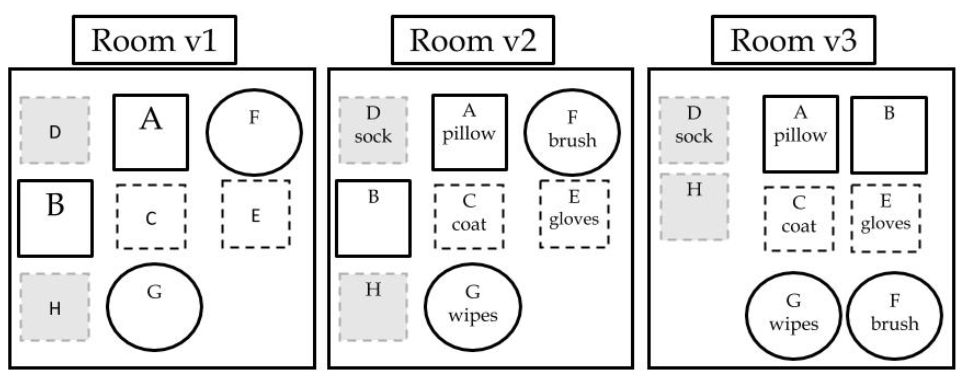
\includegraphics{C:/Users/Public/Dropbox/2-theory/1_skilled_reflection/website/figs/group.png}

\begin{enumerate}
\def\labelenumi{\arabic{enumi}.}
\setcounter{enumi}{35}
\item
  Ask what it would take to change (if possible), and whether change is worth it.
\item
  Savings occur anytime you complete an action that serves various GOALS.

  \begin{enumerate}
  \def\labelenumii{\arabic{enumii}.}
  \tightlist
  \item
    An example is Grouping (c3.35.4).\\
  \item
    Apply to IDEAs, PLANs, GOALs, or HOME things.
  \end{enumerate}
\item
  TIME is the constant (or denominator) for FORCES, FORGETTING, PRI, and LIB.

  \begin{enumerate}
  \def\labelenumii{\arabic{enumii}.}
  \tightlist
  \item
    Do not ignore TIME.
  \item
    Estimate durations accurately for GOAL accomplishment.
  \item
    Study TIME to learn reality, SELF, and their LINK.
  \item
    Continually assess whether GOAL benefits outweighs costs of TIME.
  \end{enumerate}
\item
  Maybe it seems unnecessary to represent WORK satisfaction and relationship
  quality in terms of carrots and tomatoes.
\item
  When you get bored, ask yourself why attempting to understand and define yourself bores you.
\item
  What is happening in your life, and what is in your control if these are unclear?
\item
  If you are not reflecting on your life, your garden is a foggy labyrinth, and you are a drunk gardener wearing oven-mitts.
\item
  You are pushed like a sail by any wind, the FORCES of reality.
\item
  A FORCE is any cause of change.
\item
  A FORCE underlies every action involved in a GOAL, yours or otherwise.
\item
  There are forces within your control, and forces outside.
\item
  MAINTENANCE is the COST of FORCE to neither move toward nor
  away from a GOAL.
\item
  ALIGNMENT is when NORM or natural FORCE causes your GOAL to be more likely.

  \begin{enumerate}
  \def\labelenumii{\arabic{enumii}.}
  \tightlist
  \item
    To ALIGN is to adjust your GOAL to be more like another force, usually one acting against your GOAL.
  \item
    Study how forces WORK against you.
    moment
  \end{enumerate}
\end{enumerate}

\hypertarget{now}{%
\section{Now}\label{now}}

\begin{enumerate}
\def\labelenumi{\arabic{enumi}.}
\setcounter{enumi}{46}
\tightlist
\item
  Now is the only use-case of shared space, in time.
\item
  A MOMENT is any now that is not the latest, either future or past.
\item
  A record of now becomes past `nows' of variable use-case.

  \begin{enumerate}
  \def\labelenumii{\arabic{enumii}.}
  \tightlist
  \item
    That is, we might reflect on the previous nows that we shared.
  \item
    Note that past nows do not maintain the same level of rigor. They are degraded to hype when mis-replayed, misunderstood, or accessed under changed priorities.
  \item
    In seeing passage, we might speculate on future nows to be shared.
  \item
    The discourse of past or future is always at least partially hype, but real (use) when bet on.
  \end{enumerate}
\end{enumerate}

\hypertarget{ppl}{%
\chapter{PPL}\label{ppl}}

\begin{enumerate}
\def\labelenumi{\arabic{enumi}.}
\item
  Just like you, others are trying to figure out what goes on in their own garden.* PPL are different VERSIONs of each others' PRI ({[}see also c9.70{]}{[}NORMs STYLE{]}).
\item
  Amid the goals and forces of this chapter, none of what is described includes using WORDs. Reader, you will begin to understand their nature in the next chapter, BET, but as it pertains WORDs that PPL use with each other, not until the last chapter, COMM.
\end{enumerate}

\hypertarget{places}{%
\section{Places}\label{places}}

\begin{enumerate}
\def\labelenumi{\arabic{enumi}.}
\setcounter{enumi}{2}
\tightlist
\item
  Consider PPL in terms of the four places of your life:

  \begin{enumerate}
  \def\labelenumii{\arabic{enumii}.}
  \tightlist
  \item
    on your garden dealing with your SELF.
  \item
    on someone else's garden.
  \item
    at WORK making something for others for money.
  \item
    getting something someone else made (MARKET).
  \end{enumerate}
\item
  Sometimes you are at your garden's edge
  looking elsewhere.
  For example, when you read an email or social media feed,
  as if looking across your neighbor's plot,
  studying how to bring your lettuce back to life,
  or celebrating your friend's successful pumpkin patch.
\end{enumerate}

\hypertarget{gate}{%
\section{Gate}\label{gate}}

\begin{enumerate}
\def\labelenumi{\arabic{enumi}.}
\setcounter{enumi}{4}
\tightlist
\item
  Despite garden-based PRIs, most of your time
  is spent outside your garden, and mostly for WORK (about 80,000 hours in your life).
\item
  Acknowledge the PPL in your PRIs, yet don't let them distract.
\item
  Notice how long you leave your garden and to where.
\item
  Spend only as much time needed away for your PRIs.
\item
  For example, most time on others' gardens, and any more than the minimum at WORK or MARKET is CAKE. When in doubt, go HOME and stare at your plants. At least that CAKE is free.
\end{enumerate}

\hypertarget{work}{%
\section{Work}\label{work}}

\begin{enumerate}
\def\labelenumi{\arabic{enumi}.}
\setcounter{enumi}{9}
\item
  Where do you get seeds for FOOD from and how did you know to plant them?
\item
  From other PPL, right? No silly, you don't know how to garden a sandwich!
\item
  Lucky for you, many of the most important crops you want are already grown, prepared and handed to you--in exchange for money.
\item
  Money is traded for maintenance of, or insurance for SELF and CAKE, like apples, miracle medical procedures, and a toilet to take your poop somewhere else.
\item
  WORK is performing a specific task on a collective garden, like an institution's in exchange for money. It is a pre-arranged visit to another garden for a specified time.
\item
  Whether or not you like it, or it directly fulfills garden needs, WORK is made to serve NORMS, not you.
\item
  NORMS are all actions assumed of (or about) the ``average'' person. They are the web of FORCES of all actions of all PPL, including WORK, religion, popular attitudes, and DOUBTS.
\end{enumerate}

\hypertarget{analysis}{%
\section{Analysis}\label{analysis}}

\begin{enumerate}
\def\labelenumi{\arabic{enumi}.}
\setcounter{enumi}{16}
\item
  If you have a job that pays you to think, your mind is hired to make NORMS products real.
\item
  Instead of your reality, your WORK is to translate NORMS's reality, CHUD-adjusted.
\item
  NORMS assume you will WORK for money for goods.
\item
  Language, agreed usage of WORDS, is made from NORMS.
\item
  NORMS push against individuality (except where it provides a lucrative job opportunity).
\item
  Relationships (RLTP) are GOALS about PPL (PPL).
\item
  Good ones are aligned with your GOALS.
\item
  Bad ones COST more.
\item
  A RLTP is a reciprocal pair of BETS, yours of them, and vice versa. One is the better and the other is the bet and bet on.
\item
  RLTPS, especially family members, coordinate many GOALS for SAVINGS.
\end{enumerate}

\hypertarget{others}{%
\section{Others}\label{others}}

\begin{enumerate}
\def\labelenumi{\arabic{enumi}.}
\setcounter{enumi}{26}
\item
  Maybe they are your friend, and need help with some unruly vines, or maybe you just like their apples.
\item
  Sometimes, PPL will contribute to your goals, as if bringing water to crops you didn't recognize need them. 4. Sometimes PPL will try to water your crops when they don't need watering.
\item
  Sometimes you'll return with higher morale or a bag of apples.
\item
  Sometimes you'll need to water some crops that need to be watered, because the sight of their neglect cannot be ignored.
\item
  The challenges that overwhelm you are the same for others, just not always the same amount nor at the same time.
\item
  The place, duration and impact on your PRIs are the basic measurements of a RLTP.
\item
  Pick WORK and RLTPs, including friends, that maximize your other PRIS including possibly one that maximizes TIME and money to apply to other PRIS.
\item
  Maximally ALIGN with NORMS with least compromise to PRIs. Get along with PPL.
\item
  PPL are the part of PRIs that require the most care, and fewest words.
\item
  A GOOD RLTP is a CONTRACT of the reciprocated actions (USE) between two PPL.
\item
  A BAD RLTP is HYPED mutual BETs (unaligned with actions), that waste time.
\end{enumerate}

\hypertarget{bet}{%
\chapter{Bet}\label{bet}}

\begin{enumerate}
\def\labelenumi{\arabic{enumi}.}
\tightlist
\item
  You can't help but think how to make your life better.
\item
  You can take control of your life, or you can let the world BET for you.
  You can commit yourself to finding out which thoughts are right or
  leave it to chance to have better life.
\item
  A commitment is the first step, but far from the last.
\item
  If you want your dreams to become real, listen to your DOUBTs.
\item
  Then test them.
\item
  Winning means your reality is one step toward your GOAL.
\item
  Losing is the wake-up call to be more realistic.
\item
  Betting is a protocol to guide you to reality, and, if you're lucky, your
  dreams might fit in.
\item
  How real will your dreams get before you die?
\end{enumerate}

\hypertarget{stranger}{%
\section{Stranger}\label{stranger}}

\begin{enumerate}
\def\labelenumi{\arabic{enumi}.}
\setcounter{enumi}{9}
\tightlist
\item
  A stranger comes to your garden at the end of a long day, which you realize only when you hear him chopping his jaw at you. You look up.
\item
  ``No really, consider it, right now. Imagine the most realistic, attainable, best life you could have.
\item
  Imagine taking the first step and then stay with the thought. Listen to the fear that surfaces.
\item
  For the moment, never mind how the world has gotten in your way.
\item
  How are you in your own way?''
\item
  He seems to be in your way. He's staring past your wet forehead.
\item
  ``See your DOUBTs with curiosity. Now BET on what you tell yourself
  you believe. BET on overcoming them.''
\item
  But you mostly only think of frustration and say, ``I appreciate the suggestion.''
\item
  ``Let's both BET. Name what you believe you can accomplish tomorrow, in terms of what you think holds you back most.
\item
  If you make it happen before sun-up, you'll be over the most daunting hurdle between you and your outcome.
\item
  And I'll give you the equivalent of your harvest, today. If you fail, you leave me today's harvest.''
\item
  ``Okay,'' you say. You'll show him.
\item
  ``The rocks on the far field. They're on a slippery slope. To build the home I want, I need those rocks, but I'm afraid of falling. I've collected every rock on my land and I need those rocks. Tomorrow I'll finish my foundation with rocks from the slippery slope.''
\item
  The stranger and you have set up a bet, a type of belief.
\end{enumerate}

\hypertarget{bet-1}{%
\section{BET}\label{bet-1}}

\begin{enumerate}
\def\labelenumi{\arabic{enumi}.}
\setcounter{enumi}{23}
\tightlist
\item
  A BET is a PLAN template for reconciling REALITY with CHUD, to accomplish GOALS.
\item
  Betting is confronting COSTs, HABITs, UNKNOWNs and DOUBTs that stand in the way of your wants and dreams.
\item
  The TIME that passes and the status of your GOAL when it runs out are an intersection of reality: the world and you. To name them, is to shed CHUD.
\item
  Every IDEA you hold is a BET with a rolling deadline, idiosyncratic successes, and revisions.
\item
  BET wins shorten your PLAN, and the distance to your GOAL. Losses should guide revisions to your CHUD.
\item
  To BET, name:

  \begin{enumerate}
  \def\labelenumii{\arabic{enumii}.}
  \tightlist
  \item
    a step in your PLAN,
  \item
    a deadline to achieve it, and
  \item
    the C.H.U.D. for that duration.
  \end{enumerate}
\item
  Blitz to revise and win, and log your actions.
\item
  When the deadline arrives, take stock.

  \begin{enumerate}
  \def\labelenumii{\arabic{enumii}.}
  \tightlist
  \item
    Compare your action log to your PLAN.
  \item
    Identify CHUD factors that best explain discrepancies.
  \item
    Revise PLAN, updated with CHUD factor predictions.
  \item
    (Record TIME to do the next BET or GOAL, Revise, etc.)
  \item
    Start the next BET or GOAL.
  \end{enumerate}
\end{enumerate}

\hypertarget{after}{%
\section{After}\label{after}}

\begin{enumerate}
\def\labelenumi{\arabic{enumi}.}
\setcounter{enumi}{31}
\tightlist
\item
  The next morning you woke to a field in disarray and a letter. You had
  worked harder than you planned, and still fell short of your GOAL.
\item
  ``If you did more than you would have without the BET, you won
  something, including evidence that there is some commitment in you
  to make your dreams come true.''
\item
  The biggest reward is not positive: accept you failed,
\item
  and partly due to a miscalculation.
\item
  Therefore, likely other parts of your PLAN are misguided, and your
  GOAL is further than you estimate.
\item
  If you disagree, let's BET again. First, take a minute to learn from your
  planning mistake.
\end{enumerate}

\hypertarget{c.h.u.d.}{%
\section{C.H.U.D.}\label{c.h.u.d.}}

\begin{enumerate}
\def\labelenumi{\arabic{enumi}.}
\setcounter{enumi}{37}
\tightlist
\item
  Even if you make a PLAN and BET on it, you can fail.
\item
  Why don't we achieve our GOALS?
\item
  Here are the four critical aspects of success,
\item
  and, by extension, clues for why we fail.
\item
  CHUD encompasses the changes in you, the world, and your GOAL for
  you to achieve it.
\end{enumerate}

\hypertarget{cost}{%
\section{COST}\label{cost}}

\begin{enumerate}
\def\labelenumi{\arabic{enumi}.}
\setcounter{enumi}{42}
\tightlist
\item
  COSTs (\protect\hyperlink{self-1}{c2.51}) and HABITs are knowable facts.
\item
  Observers could independently note and agree on your COSTS and HABITS.
\item
  COSTS are the unadjusted record of transactions in your life.
\item
  Referring to COST is referring to typical transactions for a GOAL.
\item
  For example, a relationship with an alcoholic poses a RISK of violence.
\end{enumerate}

\hypertarget{habit}{%
\section{HABIT}\label{habit}}

\begin{enumerate}
\def\labelenumi{\arabic{enumi}.}
\setcounter{enumi}{47}
\tightlist
\item
  The unadjusted, plain record of everything you have physically done, is your HABIT.
\item
  Referring to HABIT is referring to patterns of behavior.
\item
  For example, I eat every morning before 9 AM.

  \begin{enumerate}
  \def\labelenumii{\arabic{enumii}.}
  \tightlist
  \item
    HABITS are your most likely and reliable FOOD or CAKE actions.
  \item
    Bad HABITS are FORCES working against your GOALS.
  \item
    Good HABITS are ALIGNED with GOALS.
  \end{enumerate}
\end{enumerate}

\hypertarget{unknown}{%
\section{UNKNOWN}\label{unknown}}

\begin{enumerate}
\def\labelenumi{\arabic{enumi}.}
\setcounter{enumi}{50}
\tightlist
\item
  UNKNOWNS and DOUBTS are the gap between your real and perceived COSTs and HABITs.\\
\item
  If you have not arrived at the GOAL, there are UNKNOWNs.
\item
  UNKNOWNs are all that are fully out of your control (analogous to statistical `error').
\item
  For example, a train might stop you from arriving on TIME.
\item
  UNKNOWNs are reduced by estimating causes of failure.
\item
  For example:

  \begin{enumerate}
  \def\labelenumii{\arabic{enumii}.}
  \tightlist
  \item
    I will die, but not know how or when. The cause is UNKNOWN.
  \item
    I will die due to a natural disaster or cancer. The cause is named, and the UNKNOWN is pushed to those things' underlying causes.
  \end{enumerate}
\end{enumerate}

\hypertarget{doubt}{%
\section{DOUBT}\label{doubt}}

\begin{enumerate}
\def\labelenumi{\arabic{enumi}.}
\setcounter{enumi}{56}
\tightlist
\item
  DOUBTs are misperceptions caused or perpetuated by your HABIT.
\item
  Like COSTs, DOUBTs are the patterns of UNKNOWN.
\item
  DOUBT is any systematic error that is possible to be addressed by another human of equal ability and resources.
\item
  For example, ``self-fulfilled prophesies'', irrational fear or anxiety.\\
\item
  Good DOUBTS temper an optimistic PLAN.
\item
  Otherwise (Bad) DOUBTS:

  \begin{enumerate}
  \def\labelenumii{\arabic{enumii}.}
  \tightlist
  \item
    fuel bad HABITs and fantasies.
  \item
    Like Fear, anxiety, and jealousy, reflect overestimations.
  \item
    Like narrow-mindedness, reflect underestimations.
  \item
    Like distraction and boredom can be:

    \begin{enumerate}
    \def\labelenumiii{\arabic{enumiii}.}
    \tightlist
    \item
      anxiety about your future.
    \item
      discomfort toward present reality.
    \item
      distrust in your past.
    \end{enumerate}
  \end{enumerate}
\item
  Most of these issues, if deep enough, require therapy.
\item
  Or the {[}Intellectual Bootcamp{]}.
\end{enumerate}

\hypertarget{the-i.b.c.}{%
\chapter*{The I.B.C.}\label{the-i.b.c.}}
\addcontentsline{toc}{chapter}{The I.B.C.}

\hypertarget{education}{%
\chapter{Education}\label{education}}

\hypertarget{the-classroom}{%
\section{The Classroom}\label{the-classroom}}

\begin{enumerate}
\def\labelenumi{\arabic{enumi}.}
\tightlist
\item
  A CLASSROOM is a special case of MARKET and WORK; the direct and
  shared exchange of mental work, for the purpose of improving
  individual PRIs.
\item
  No one chose to be born. Everyone begins life with their own unnamed
  and unanswered problems.
\item
  Books are an author's answers; they can only tell a student what the
  answer is not (quite).
\item
  Instead of teaching how to read between the lines, let the student
  define the problem through their reality and life GOALS.
\item
  Let them write the PLAN and teach them only what is needed to
  succeed.
\item
  Imagine a perfect course exists, designed to teach you to fulfill
  your specific ambitions.
\item
  Every aspect of what you NEED to know, that is known and
  communicable, is the only thing written.
\item
  Everything that cannot be known but must be discovered or practiced,
  is laid out as a set of instructions, described in the WORDS that
  maximize the learning opportunity, and your progress.
\item
  Rather than a course in a classroom, the perfect class is a manual
  to reference as you live your life, or at least until you've
  internalized its contents:
\item
  when to take a break to strategize your decisions, lessons on what
  opportunities to watch for and resist, and so on.
\item
  Any social role you wish to take on, artist, engineer, therapist,
  insurance salesperson, reliable partner, is customized intimately,
  curated perfectly for what you need.
\item
  Any RLTP or interpersonal skill that is realistically possible for
  you is preceded with the guidance and education that prepares you
  emotionally to choose the right experiences that set you up to be
  most likely to find and make the most of opportunities to share
  yourself with another.
\end{enumerate}

\hypertarget{prompt}{%
\section{Prompt}\label{prompt}}

\begin{enumerate}
\def\labelenumi{\arabic{enumi}.}
\setcounter{enumi}{12}
\tightlist
\item
  Is there a better version of you?
\item
  Are you capable of moving toward it?
\item
  Are you ready?
\item
  If your answers are yes, then you are a student. To live a better
  life, you will commit to change your actions.
\item
  First, you will learn what changes are needed.
\end{enumerate}

\hypertarget{admissions}{%
\section{Admissions}\label{admissions}}

\begin{enumerate}
\def\labelenumi{\arabic{enumi}.}
\setcounter{enumi}{17}
\tightlist
\item
  This is a boot camp whose purpose is

  \begin{enumerate}
  \def\labelenumii{\arabic{enumii}.}
  \tightlist
  \item
    to train adults to think harder, clearer and more effectively.
  \item
    to produce intelligent solutions for personal and social
    puzzles.
  \item
    to have a higher cognitive discipline.
  \item
    to instill shared CAKE about reason, thinking and discourse.
  \item
    to empower.
  \end{enumerate}
\item
  It is a training program designed to break down bad habits of
  thought, and build good ones while immersed here, a culture of
  rational thinking isolated from the outside world.
\end{enumerate}

\hypertarget{challenge}{%
\section{Challenge}\label{challenge}}

\begin{enumerate}
\def\labelenumi{\arabic{enumi}.}
\setcounter{enumi}{19}
\tightlist
\item
  Here you will relentlessly confront your ideas about the world, with
  instructors drilling intellectual skills (writing essays, arguing
  for ideas, and developing proposals for action).
\item
  You will be trained to move toward your GOALS with focus, even in
  the face of perceptual, physical, or emotional distractions.
\item
  Over TIME, students could expect to cultivate a sharper focus on
  cognitive objectives, resilience to distractions and challenges.
\item
  If you graduate, it will be with the ability to identify, develop,
  and communicate ideal critical, rational arguments, positions or
  PLANS (orally or written) given the available knowledge, finite
  TIME, and resources at hand (reference material, teamwork).
\item
  you will also learn a code of behavior for being a community leader,
\item
  collaborating or competing with an irrational world.
\item
  The central requirement for applicants will be a commitment to
  better understand the SELF and world.
\end{enumerate}

\hypertarget{student}{%
\section{Student}\label{student}}

\begin{enumerate}
\def\labelenumi{\arabic{enumi}.}
\setcounter{enumi}{26}
\tightlist
\item
  Students are PPL with IDEAS from EXPERIENCE toward selfish GOALS.
\item
  Lessons depend on students' prior knowledge.
\item
  A STUDENT

  \begin{enumerate}
  \def\labelenumii{\arabic{enumii}.}
  \tightlist
  \item
    has a GOAL that can be better named and planned.
  \item
    requires TIME away from BETTING.
  \item
    admits not knowing but capable.
  \end{enumerate}
\item
  Students learn to represent their knowledge in WORDS; to prefer
  better, alternative WORDS. A student sees the impersonal as more
  reliable both for selfish GOALS and social ones.
\item
  A bad student studies to avoid action, or for its own sake.
\item
  A Student WRITES IDEAs and GOALS to their INSTRUCTOR.
\item
  Your GOAL is clear. You want:

  \begin{enumerate}
  \def\labelenumii{\arabic{enumii}.}
  \tightlist
  \item
    The strength needed to take the right steps and make a habit of
    it,
  \item
    keen eyes to estimate the destination and correct course, and
  \item
    a focused mind to steady the foot.
  \end{enumerate}
\end{enumerate}

\hypertarget{consent}{%
\section{Consent}\label{consent}}

\begin{enumerate}
\def\labelenumi{\arabic{enumi}.}
\setcounter{enumi}{33}
\tightlist
\item
  This is an in-person immersive experience.
\item
  You only really learn what you need to know to be who you really
  want. You won't learn unless you cannot escape needing it; in a
  dedicated environment that fosters acquisition, minimizes
  interference.
\item
  Whether you're here for the 7- or 30-day experience, you will WORK
  hard every minute.
\item
  For every minute of lesson on my TIME, students are to provide two
  minutes of writing, either toward others' learning or in direct
  application toward their GOAL.
\end{enumerate}

\hypertarget{course}{%
\section{Course}\label{course}}

\begin{enumerate}
\def\labelenumi{\arabic{enumi}.}
\setcounter{enumi}{37}
\tightlist
\item
  Dedicate to identity growth. Be:

  \begin{enumerate}
  \def\labelenumii{\arabic{enumii}.}
  \tightlist
  \item
    Quiet, except when tasks require verbal response.
  \item
    Receptive to WORK and feedback provided by the instructor.
  \item
    Committed to producing genuinely inspired ideas, working
    quickly, and seeking improvement.
  \item
    Respectful that all are equal in voice, and aim to describe
    solutions with collective CAKE.
  \item
    Receptive and responsive to prompts and observations (from peers
    and/or instructors) especially CHUD, vague language, and
    cognitive bias.
  \item
    Motivated to describe solutions that benefit others, when
    possible, including peer-review.
  \end{enumerate}
\item
  Learn:

  \begin{enumerate}
  \def\labelenumii{\arabic{enumii}.}
  \tightlist
  \item
    Precisely and only what is needed to trust a clear picture of
    what your life is.
  \item
    First, how to make a PLAN, a map of who you are, and who you
    want to be;
  \item
    Repeat Part one of this book, until your PLAN is good enough to
    be wrong, and truthful enough to hurt.
  \end{enumerate}
\item
  This will be the beginning of change, and the first test of your
  commitment.
\item
  Your performance is evaluated simply: whether or not you
\item
  end up eating, sleeping, thinking, talking, and acting differently.
\end{enumerate}

\hypertarget{think}{%
\section{Think}\label{think}}

\begin{enumerate}
\def\labelenumi{\arabic{enumi}.}
\setcounter{enumi}{42}
\tightlist
\item
  Think, student.
\item
  Do not take notes, simply pay attention.
\item
  Everything I say is meant plainly.
\item
  If you get confused, forget it, and pay attention to right now.
\item
  Our GOAL here is thinking. Thinking happens in your heads.
\item
  Right now your job is to think about the truth you see in what i
  say.
\item
  A student has two roles to think in: Reader and Writer.
\end{enumerate}

\hypertarget{read}{%
\section{READ}\label{read}}

\begin{enumerate}
\def\labelenumi{\arabic{enumi}.}
\setcounter{enumi}{49}
\tightlist
\item
  Read, student.
\item
  A reader is a listener and observer.
\item
  Reading is the same as listening to an instructor,
\item
  except that the speaking pace doesn't determine how fast you have to
  think, or remind you to
\item
  pay attention!

  \begin{enumerate}
  \def\labelenumii{\arabic{enumii}.}
  \tightlist
  \item
    Your attention cannot be trusted on its own,
  \item
    so lose distractions
  \item
    like your smart phone.
  \item
    You will befriend the simplest scientific instrument, a clock.
  \item
    The clock is a cue to think.
  \item
    When it goes off, get back on task.
  \item
    The clock will babysit your unreliable attention.
  \end{enumerate}
\end{enumerate}

\hypertarget{truth}{%
\section{Truth}\label{truth}}

\begin{enumerate}
\def\labelenumi{\arabic{enumi}.}
\setcounter{enumi}{54}
\tightlist
\item
  Your GOAL in reading is to isolate the truth from the lie.

  \begin{enumerate}
  \def\labelenumii{\arabic{enumii}.}
  \tightlist
  \item
    Try reading this sentence:
  \item
    ``Everyone is best off running weekly until they die.''
  \item
    You're thinking, ``this can't be true for everyone, so it's a
    lie.''
  \item
    Not so fast.
  \item
    There are many components to this idea, and likely many that you
    believe are truthful.
  \item
    Often a lie becomes true just by changing the pronouns in the
    text.
  \item
    Consider this revision: ``I am best off running weekly until I
    die.''
  \item
    Perhaps now the WORDS are more truthful to you.
  \end{enumerate}
\item
  Doing this makes a clear relationship between your belief and the
  author's.
\item
  Becoming smart is the discipline of understanding how you relate to
  others.
\item
  When reading, dismiss only what you fully believe is an intentional
  lie.
\item
  More generally, read to assess your BET on the WORDS reflecting
  TRUTH.
\item
  Whether to a single WORD, a line, chapter, or book.
\item
  Assign WEIGHTs (0 to 9) to what you read, to complete this prompt:
\item
  I BET this is true for:

  \begin{enumerate}
  \def\labelenumii{\arabic{enumii}.}
  \tightlist
  \item
    0 = not even the author.
  \item
    1 = only the author.
  \item
    2 = the author, me, and a few others.
  \item
    3 = Us and 30\% of everyone else.
  \item
    9 = Us and about 90\% of everyone else.
  \end{enumerate}
\item
  For every assertion and assumption you read, begin assuming it is a
  ``9'', working backwards according to evidence you hold.
\end{enumerate}

\hypertarget{lesson}{%
\section{Lesson}\label{lesson}}

\begin{enumerate}
\def\labelenumi{\arabic{enumi}.}
\setcounter{enumi}{63}
\item
  The following mini lesson illustrates the risk at hand--involuntary
  comprehension, and the benefit at stake from deliberate reading.
\item
  Consider the following quote, ``Change your thoughts to change your
  life.''
\item
  Comprehension is involuntary.

  \begin{enumerate}
  \def\labelenumii{\arabic{enumii}.}
  \tightlist
  \item
    You cannot help but recognize meaning when you read.
  \item
    This means that you likely thought the quote was largely
    unrealistic.
  \end{enumerate}
\item
  Reading as proposed here, is strongly voluntary.
\item
  For example, reread the quote, this TIME assuming it is reasonable,
  serious, and valuable.
\item
  The statement is the core assumption to this book, and any
  psychological theory.
\item
  For example, Freud's talk therapy was, in his TIME, the radical idea
  that WORDS could fix PPL.
\item
  Therefore, do not waste the opportunity to consider a truth that
  could change your life by failing to entertain a simple assumption.
\end{enumerate}

\hypertarget{say}{%
\section{Say}\label{say}}

\begin{enumerate}
\def\labelenumi{\arabic{enumi}.}
\setcounter{enumi}{71}
\tightlist
\item
  How will your life look if you put it on paper? Like a bunch of
  WORDS.
\item
  How do you change it? By deleting the WORDS with lies, and replacing
  them with better WORDS.
\item
  The right WORDS will change your actions and your life. To live a
  better life, starts with your WORDS.
\item
  In order to do something about thoughts, we need to think on paper.
  {[}You'll write a lot. You'll delete a lot. You'll get good at
  writing.{]}
\end{enumerate}

\hypertarget{write}{%
\section{WRITE}\label{write}}

\begin{enumerate}
\def\labelenumi{\arabic{enumi}.}
\setcounter{enumi}{75}
\tightlist
\item
  BET on WORDS. A writer invests TIME and energy to map feelings onto
  WORDS.
\item
  Good writing is discovering, curating, and applying insight. Bad
  WRITING has an author; ad hominem.
\item
  Revisions also make you a WRITER. When you revise WORDS (yours or
  others') to maximize your BET, you are a writer.
\item
  Separate thought and SELF (author), by BETTING explicitly.
\item
  State your assumptions, do not justify them. -is-STYLE-bad
\item
  Replace ``I am.'' with tag WORDS.
\item
  Strive for COMM-CONTENT and brevity; Write only valuable BETs, or
  WORDS that manifest valuable BETs. Prioritize understanding over
  original writing.
\item
  WRITING for LIB-PPL, relatable, depersonalized, objective WORDS,
  minimizes rot, maximizes PLAN utility.
\end{enumerate}

\hypertarget{instructor}{%
\section{Instructor}\label{instructor}}

\begin{enumerate}
\def\labelenumi{\arabic{enumi}.}
\setcounter{enumi}{83}
\tightlist
\item
  I am an instructor, a guardian of true IDEAs and WRITER of a general
  PLAN (this book).
\item
  An instructor READS, and enforces BETs on LINKs toward a PLAN.
\item
  My GOALS are to

  \begin{enumerate}
  \def\labelenumii{\arabic{enumii}.}
  \tightlist
  \item
    Minimize student effort and TIME to write.
  \item
    READ for cognitive biases, illogical appeals, and imprecise
    language, and WRITE feedback that is dispassionate and neutral,
    yet invested and True.
  \item
    Reward arguments based on (Truth:) REALITY, SELF, and CAKE.
  \item
    Reward IDEAS shared (vs kept).
  \end{enumerate}
\end{enumerate}

\hypertarget{answers}{%
\section{Answers}\label{answers}}

\begin{enumerate}
\def\labelenumi{\arabic{enumi}.}
\setcounter{enumi}{86}
\item
  Which lines from this book would you {[}BET on{]}{[}How to Read{]}, written
  as-is, or revised for you?
\item
  Assign 100 dollars (total) to those lines according to their
  relative impact, and you are an IBC student; an author of shared
  truth.
\item
  Suppose a representative set of PPL did the same thing. Here's a
  game to help imagine.

  \begin{enumerate}
  \def\labelenumii{\arabic{enumii}.}
  \tightlist
  \item
    Each student's bets go to a general pool.
  \item
    When bets on a line reach a critical mass, the pool of sub-par
    bets is split among winners.
  \item
    Cash is divided.
  \item
    Also, points are recorded, to incentivize a deeper purpose:
  \item
    A game, where the prize is
  \item
    the collective revision and authorship of this book.
  \item
    After x wins, your name appears on the title.
  \item
    High scores are on the acknowledgements page.
  \item
    This is the process and meaning of READER and WRITER; bound
    directly to material and action, IRL.
  \end{enumerate}
\item
  Whereas the exchange of MONEY incentivizes the revision of truth,
  the CONTENT itself would be the premise to the next book, {[}the
  Answerword{]}{[}The Answerword{]}.
\end{enumerate}

\hypertarget{words}{%
\chapter{WORDS}\label{words}}

\hypertarget{cognition}{%
\section{Cognition}\label{cognition}}

\begin{enumerate}
\def\labelenumi{\arabic{enumi}.}
\tightlist
\item
  WORDS describe the world and its conditions.
\item
  This chapter is about problems and answers regarding the ACT of
  describing, itself:

  \begin{enumerate}
  \def\labelenumii{\arabic{enumii}.}
  \tightlist
  \item
    WORDS said do not usually reflect what PPL want or need.
  \item
    By engaging the gap between WORDS and reality, you increase
    SELF-awareness (BET).
  \item
    Better WORDS mean more practical understanding and expectations,
    more complete desires, and
  \item
    The capacity to make a concrete PLAN for achieving your GOALS.
  \item
    This will include healthier COMM and RLTPs.
  \item
    A community with better WORDS has clearer idea sharing,
    synthesizing, developing, teaching and learning.
  \end{enumerate}
\end{enumerate}

\hypertarget{problem}{%
\section{Problem}\label{problem}}

\begin{enumerate}
\def\labelenumi{\arabic{enumi}.}
\setcounter{enumi}{2}
\tightlist
\item
  Speaking your mind is difficult to do accurately.
\item
  A memory system dealing with language is tasked to translate
  thoughts into the right WORDS from tens of thousands. It is prone to
  inaccuracies.
\item
  Similarly, a listener focused on comprehending, is not likely to
  monitor all the incidental priming effects of WORDS on a memory
  system.
\item
  WORDS said and heard impact both parties' beliefs and behaviors.
\item
  Saying WORDs or Hearing and understanding a WORD is a very small
  physical action, to describe real actions and consequences.
\item
  The issue is that WORDs can be more and less right, more and less
  helpful, and without intervention, it is very difficult to know how
  much this is true in any example of WORD USE.
\item
  Bad WORDS keep CHUD expensive and waste TIME.
\item
  The COST of an individual WORD is tiny, but we say tens of thousands
  per day (Levelt).
\end{enumerate}

\hypertarget{bet-2}{%
\section{Bet}\label{bet-2}}

\begin{enumerate}
\def\labelenumi{\arabic{enumi}.}
\setcounter{enumi}{10}
\item
  A GOOD general BET about WORDs is to begin assuming every WORD is a
  BET on hypotheticals, which can be true (reality) or false
  (fantasy).
\item
  A PLAN is a BET on a winning arrangement of WORDS that result in the
  GOAL.
\item
  Reading, thinking, saying, and writing a WORD perpetuates that
  WORD's IDEA over others, either moving you toward a GOAL, or your
  HABIT.
\end{enumerate}

\hypertarget{simulation}{%
\section{Simulation}\label{simulation}}

\begin{enumerate}
\def\labelenumi{\arabic{enumi}.}
\setcounter{enumi}{13}
\item
  WORDS efficiently simulate possible worlds. You can think through
  far more situations with WORDS, than you can (or should) act out.
\item
  Your GOALS can be described in WORDS, and WORDS can be easily
  crossed out and revised.
\item
  Good WORDS maximize productivity of thought, move you beyond
  pitfalls of CHUD, direct attention to PRIS, and predict reality;
  improve decisions and make you smarter.
\item
  By thinking about all WORDS you experience (LIB), you can take
  control to limit your WORD use toward more productive ones,
  improving READ and WRITE decisions, increasing focus and TIME for
  GOALS.
\item
  SIM (F-ACT) is the act of iterating between WRITE and READ, to evoke
  and NAME the optimal, held BET. Tour SIM is not constrained by IRL,
  but your picture of IRL, and your SIM GOAL is to capture the picture
  true to your CHUD estimate.
\end{enumerate}

\hypertarget{it}{%
\section{``It''}\label{it}}

\begin{enumerate}
\def\labelenumi{\arabic{enumi}.}
\setcounter{enumi}{18}
\item
  It caused you to NAME in the first place. This cause is ``IT''.
  GOOD-REF is giving the best NAME for our desired COMM.
\item
  For example, take these background facts, which contains the basis
  of our desired REF.

  \begin{enumerate}
  \def\labelenumii{\arabic{enumii}.}
  \tightlist
  \item
    I woke at 8:30AM
  \item
    I wanted to sleep until 9:30AM.
  \item
    In my 9:00AM appointment with you, as you are talking, I yawn.
  \item
    You say, ``I must be boring you.''
  \item
    I want to hear what you were going to say (COMM-PRI).
  \end{enumerate}
\item
  Each of these (below) are slightly different REFs based on the facts
  (above), ranked by GOOD-REF:

  \begin{enumerate}
  \def\labelenumii{\arabic{enumii}.}
  \tightlist
  \item
    You're not, please continue.
  \item
    No, I'm tired.
  \item
    No, I woke early.
  \item
    Don't make assumptions.
  \item
    I'm not.
  \item
    ``I woke at 8:30AM, but wanted to sleep until 9:30AM, so I think
    I yawned because I am tired.''
  \item
    ``I yawned because I am tired. I can see why you thought I was
    bored, and I'm sorry.''
  \item
    {[}Nothing{]}
  \end{enumerate}
\item
  All of the REFs above combined suggest the ``IT'' you want to convey.
\item
  A GOOD-REF is the one that uses truth to focus and advance the
  COMM-PRI.
\item
  Below are the REF attributes that make each choice unique (and less
  GOOD).
\item
  Give a simple reason to return to the COMM-PRI (example 1 above).
\item
  Does not add to COMM-PRI nor return to it. 3-`early' may not be
  true.
\item
  Focus on others' mistake and issue a command.
\item
  Begs the question.
\item
  Focus on the distraction.
\item
  Focus on the distraction and makes the same kind of REF which the
  other did and which caused the confusion.
\item
  This can be anywhere in the list including 1, depending on what you
  DO or SAY next.

  \begin{itemize}
  \tightlist
  \item
    1: you or the other return to COMM-PRI without ever returning to
    this interruption.
  \item
    4: it reduces the number of words said before returning to
    COMM-PRI.
  \item
    8: the distraction is remembered, and mentioned again, later.
  \end{itemize}
\item
  Let this characterize the problem and approach, and I will end with
  a few primary objectives, besides.

  \begin{enumerate}
  \def\labelenumii{\arabic{enumii}.}
  \tightlist
  \item
    GOOD-REF is a plain IDEA or LINK.
  \item
    If ``GOOD-REF'', the IDEA, crosses your mind while considering
    what to say, likely that it is a LINK.
  \item
    DECIDE and SAY REF within a few seconds, rather than THINKING
    more, unless the BET is obvious and worthwhile.
  \item
    BEST-REF is possible, but requires extra THINKING to know the
    valuable cause. This is not practical, so we go for conservative
    GOOD-REF.
  \item
    In USE, this means quickly NAME the relevant LINKs, and estimate
    the central or critical LINK between them.
  \end{enumerate}
\item
  In our example of the facts, above,

  \begin{enumerate}
  \def\labelenumii{\arabic{enumii}.}
  \tightlist
  \item
    1 is not obvious and adds little to 3.
  \item
    5 is the COMM-PRI, and 4 is the cause, but not IT in what you
    say.
  \item
    2 and 3 are IT, and specifically, the LINK between them.
  \end{enumerate}
\item
  Unless you are a RECRUIT, to go any further will usually not be
  worth the COST. To go further is to specify what kind of link is
  between the two. WANT is HYPE, etc.
\item
  GOOD-REF is ``NEW'' vs GIVEN.
\end{enumerate}

\hypertarget{write-plan}{%
\section{Write-Plan}\label{write-plan}}

\begin{enumerate}
\def\labelenumi{\arabic{enumi}.}
\setcounter{enumi}{35}
\tightlist
\item
  Speak, write, initiate or respond only in limited duration and WORDS
  dictated by intended outcome.
\item
  Use WORDS empirically, with a comparison group (vs) and quantity in
  mind.
\item
  Ideas are more important than authorship.
\item
  Do not use a WORD that is more of a Lie.
\item
  Say the truth or be quiet.
\item
  Use WORDS for decisions, not emotions.
\item
  Use WORDS to facilitate PRIS. Do not write PLANS you won't follow.
\item
  Stop talking when action (or listening) is needed.
\end{enumerate}

\hypertarget{read-plan}{%
\section{Read-Plan}\label{read-plan}}

\begin{enumerate}
\def\labelenumi{\arabic{enumi}.}
\setcounter{enumi}{45}
\tightlist
\item
  Listen / read when you need to learn / connect.
\item
  Limit duration/WORDS needed to assess consent.
\item
  Distrust ego, and take nothing personally
\item
  Investigate the empirical CAKE of WORDS.
\item
  Revise to believe, and revise PLANS into ones you'd follow.
\item
  Remove / ignore style.
\item
  Assert boundaries against exaggerated WORDS or unreliable ones.
\end{enumerate}

\hypertarget{types}{%
\section{Types}\label{types}}

\begin{enumerate}
\def\labelenumi{\arabic{enumi}.}
\setcounter{enumi}{46}
\tightlist
\item
  A description of the kinds of simulation a word can make, and the
  kinds to prioritize.
\end{enumerate}

\hypertarget{example}{%
\section{EXAMPLE}\label{example}}

\begin{enumerate}
\def\labelenumi{\arabic{enumi}.}
\setcounter{enumi}{44}
\tightlist
\item
  An EXAMPLE is an individual, particular event or object, of reality.

  \begin{enumerate}
  \def\labelenumii{\arabic{enumii}.}
  \tightlist
  \item
    An example with consequence is a USE-CASE.
  \item
    An example in-principle is a HYPE (hypothetical/hype).
  \item
    In COMM, EXAMPLES are described per the criteria that might
    support a USE of an EXAMPLE.
  \end{enumerate}
\item
  WORDS are one of two types:

  \begin{enumerate}
  \def\labelenumii{\arabic{enumii}.}
  \tightlist
  \item
    LINKS: WORDS that give relationship between EXAMPLES, IDEAS,
    describe ACTIONS, ROLES, and transformations.
  \item
    IDEAS: WORDS that refer to EXAMPLES.
  \item
    An IDEA is a set of criteria that LINK EXAMPLES as similar (vs
    not).
  \item
    The most basic IDEA classifies EXAMPLES as A or not-A. ``blue'' is
    an IDEA that certain colored things are BLUE (A), and all other
    colors are not BLUE.
  \item
    Good IDEAS group EXAMPLES in a way that directs attention toward
    PLANS and GOALS. Bad IDEAS distract.
  \item
    The right LINK between ideas is the foundation of every thought,
    RECIPE or terrible calculation.
  \end{enumerate}
\end{enumerate}

\hypertarget{hype}{%
\section{HYPE}\label{hype}}

\begin{enumerate}
\def\labelenumi{\arabic{enumi}.}
\setcounter{enumi}{46}
\tightlist
\item
  HYPE vs USE-CASE guides what and if to write. A GOAL is a named
  HYPE. GOOD HYPE are worthwhile GOALs, sub-GOALs, or ALT PLAN ACTIONs
  to consider. Don't WRITE HYPE without a BET.
\item
  As all words should be toward PRIs, there are three general modes of
  PRI WORDs:

  \begin{enumerate}
  \def\labelenumii{\arabic{enumii}.}
  \tightlist
  \item
    h0 = history. HABIT is to history as action is to DOC. GOOD
    history is structured data of your HABIT, expressly for the
    purpose of revising future actions.
  \item
    h1 = plan (pri.txt, proj\_doc.txt)
  \item
    h2 = doubt especially for bet.
  \end{enumerate}
\end{enumerate}

\hypertarget{alternatives}{%
\section{Alternatives}\label{alternatives}}

\begin{enumerate}
\def\labelenumi{\arabic{enumi}.}
\setcounter{enumi}{48}
\item
  ALTs are any IDEA which measurably deviates a PLAN, and are defined
  directly with respect to the target IDEA.
\item
  For example, BAD is an ALT to GOOD, as in ``GOOD-vs-BAD''.
\item
  Any other valid modes, if at all, are in support of maximal revision
  in these primary ones.
\item
  A PLAN comprises: 1.the decided action 2.the best bet on it
  3.alternative actions 4.the goal 5.the relevant CHUD
\item
  GOOD GOALs and their PLANs are supported by USEs from your own
  history (SELF-H), and next best is NORM or OTHERS' USE or DATA that
  generalizes.
\item
  For example, a plan for a similar goal has previously succeeded.
\end{enumerate}

\hypertarget{letters}{%
\section{Letters}\label{letters}}

\begin{enumerate}
\def\labelenumi{\arabic{enumi}.}
\tightlist
\item
  Mnemonics are memory aids.
\item
  Reducing a word to a letter increases cognitive efficiency, as long
  as that letter stands for an idea you will frequently encounter.
\item
  These letters illustrate kinds of word usage (not exhaustive):

  \begin{enumerate}
  \def\labelenumii{\arabic{enumii}.}
  \tightlist
  \item
    \texttt{f} define; function\\
  \item
    \texttt{i} synonym, sense, ``i.e.'', ``as in'',\\
  \item
    \texttt{e} example, data-point, untested data\\
  \item
    \texttt{h} history (implied h0)
  \item
    \texttt{h1} claim, thesis. vs h0 or h2.
  \item
    \texttt{x} Cross-references, xref\\
  \item
    \texttt{d} Data or evidence, summary
  \item
    \texttt{v} version / revise\\
  \item
    \texttt{vs} an alternative, sibling of a shared parent category.
  \end{enumerate}
\end{enumerate}

\hypertarget{notes}{%
\section{NOTES}\label{notes}}

\begin{enumerate}
\def\labelenumi{\arabic{enumi}.}
\setcounter{enumi}{3}
\item
  Good NOTES clarify PRI (CONTENT) within BETS from secondary ones.
\item
  In a DOC, PAR is a GROUPED set of WORDs roughly equivalent to a
  complex sentence.
\item
  It has a primary subject and predicate, and includes any immediately
  relevant branches from either.
\item
  In practice it is between 1 and 4 clauses.
\item
  GOOD PAR successfully denotes a LINK between two IDEAs, with the
  following FORM:

  \begin{enumerate}
  \def\labelenumii{\arabic{enumii}.}
  \tightlist
  \item
    a syntactic tree, where\\
  \item
    {[}newline{]} is the right path in a fork,\\
  \item
    first indent ('' -``) is the left path in a fork,\\
  \end{enumerate}

  \begin{itemize}
  \tightlist
  \item
    trailing''-'' denotes all subsequent lines in section are equal
    childs.\\
  \end{itemize}

  \begin{enumerate}
  \def\labelenumii{\arabic{enumii}.}
  \setcounter{enumii}{3}
  \tightlist
  \item
    subsequent newline indents or in-line ``--'' are siblings\\
  \item
    left to right are siblings\\
  \item
    double linebreak ends the local tree.
  \end{enumerate}
\item
  When word order is a left-to-right walk of a right-branching
  syntactic tree, sentence can be written in lines of random lengths,
  and read equally as unambiguously.
\item
  Restrict reference and vocabulary to Simple- or Plain- English to
  reduce amibiguity.
\end{enumerate}

\hypertarget{transparent}{%
\section{Transparent}\label{transparent}}

\begin{enumerate}
\def\labelenumi{\arabic{enumi}.}
\item
  Make folder and file names i-goals as transparent as possible imply
  or reveal its (hidden) members.
\item
  Promote or consolidate high frequency items or only-childs.
\item
  For example: \texttt{ppl-work\ -\textbackslash{}\textgreater{}\ work\ -\ self-home\ -\textbackslash{}\textgreater{}\ home}
\item
  When creating or reusing a word for new applications, this principle
  should be a factor.
\end{enumerate}

\hypertarget{recipe}{%
\section{RECIPE}\label{recipe}}

\begin{enumerate}
\def\labelenumi{\arabic{enumi}.}
\setcounter{enumi}{34}
\tightlist
\item
  A Recipe is one of the best ways to arrange PLANS.
\item
  Lessons and instructions use a RECIPE format.
\item
  The RECIPE format highlights the IDEAS and LINKS of your point and
  minimizes excessive STYLE.

  \begin{enumerate}
  \def\labelenumii{\arabic{enumii}.}
  \tightlist
  \item
    List key IDEAS.
  \item
    Describe actions and transformations (LINKS).
  \end{enumerate}
\item
  Given an IDEA, estimate relevance to PRIS, problems, undeveloped
  PLANS, and SELF-MAINTENANCE.
\item
  Keep docs short enough that the title and CONTENT address only one
  thing.
\item
  Save selectively and
\item
  delete frequently.
\end{enumerate}

\hypertarget{document}{%
\section{Document}\label{document}}

\begin{enumerate}
\def\labelenumi{\arabic{enumi}.}
\item
  A word is a doc when it is saved with a name, at least once.

  \begin{enumerate}
  \def\labelenumii{\arabic{enumii}.}
  \tightlist
  \item
    Word is to a GOOD DOC (for example, a resume), as action is to
    goal.
  \item
    To a BAD DOC, a word (for example a diary entry) is to an
    unnecessary purchase at a tupperware party.

    \begin{enumerate}
    \def\labelenumiii{\arabic{enumiii}.}
    \tightlist
    \item
      Notes are words for comm.
    \item
      Lib is what words to save.
    \item
      Revision is words for pris.
    \end{enumerate}
  \end{enumerate}
\item
  Introduce ideas in unambiguous terms.

  \begin{enumerate}
  \def\labelenumii{\arabic{enumii}.}
  \tightlist
  \item
    introducing a new topic, provide a succinct, distinctive
    illustration of the point or merit, \emph{in the verbiage you will
    most likely understand}.
  \item
    then describe the link with a taxonomic reference, as follows,
    where each idea read left to right is a type of or label for the
    preceding category, implying alternatives at each level.
    e-psych-teach-2021-unit4-hw-methods\_report-intro ``For this
    assignment, consider your grandparents.''
  \end{enumerate}
\item
  Illustrate the link.

  \begin{enumerate}
  \def\labelenumii{\arabic{enumii}.}
  \tightlist
  \item
    At a micro-scale, every dash itself is a link.
  \item
    For example, in the taxonomy, ``Psych-teach-2021-unit4'' the three
    latter IDEAS qualify the topic, PSYCH. The order of terms from
    left to right should closely correspond to the order of relevant
    conditional differences that determine:

    \begin{enumerate}
    \def\labelenumiii{\arabic{enumiii}.}
    \tightlist
    \item
      the pri for the reader. answer: what are the fewest words to
      help a reader know a topic is irrelevant or truly
      beneficial?
    \item
      the most similar and relevant concepts to most distinct,
      rare, and particular to what is being described.
    \end{enumerate}
  \item
    the left-most word will be either implied or actual chapter
    headings.
  \item
    All science that is not directly relevant elsewhere, will fall
    under PPL-WORK or SELF-HOME.
  \item
    The remaining chapters deal with modes on these basic sources:
    PRI and ED concern optimizing life. (What about WORD, REVISION,
    COMM?)
  \item
    In the example above, PSYCH might fall under SELF-BODY,
    SELF-HOME, PPL, PPL-WORK. Here, we are talking about defining
    links for purposes of reducing ambiguity.
  \item
    The link is the decision of the sentence that requires the most
    care. It is simply a bridge, and as such has a basic and plain
    function.
  \item
    Named links are ACTIONS.
  \item
    Over-spelling the IDEAs leaves an empty link, e-``do\ldots(the
    trash)'' consider what is the manner of spending time, if an
    action, to ascribing your link. Consider the specific change
    being undertaken. Some ACTIONS: TAKE, GIVE, MAKE, BUY, SELL,
    USE/EAT, WORK, WRITE, READ. - Notice these are all verbs of
    transfer.
  \item
    In instr, the link comes last, and it describes a step in
    revision.
  \end{enumerate}
\item
  Contextualize with an alternative

  \begin{enumerate}
  \def\labelenumii{\arabic{enumii}.}
  \tightlist
  \item
    A plan should inherit or give definitions of new terms.
  \item
    New definitions should especially be accompanied by a true
    use-case, to protect against a false problem.
  \item
    A pri is the motive for life, and itself is only a named
    spending of time.
  \item
    A developed pri is an instruction.
  \item
    One generalized is a lesson.
  \end{enumerate}
\end{enumerate}

\hypertarget{scientist}{%
\section{Scientist}\label{scientist}}

\begin{enumerate}
\def\labelenumi{\arabic{enumi}.}
\setcounter{enumi}{46}
\item
  A scientist works to win BETS against the UNKNOWN. They are a
  professional writer, evaluated on two metrics:

  \begin{enumerate}
  \def\labelenumii{\arabic{enumii}.}
  \tightlist
  \item
    For their new CONTENT.
  \item
    The net benefit on GOAL outcomes.
  \end{enumerate}
\item
  A scientist-researcher is a WRITER, a data-collector and hypothesis
  tester.
\item
  A scientist-scholar is a READER, curating toward theory development
  and COMM.
\item
  More will be said about SCIENTIST more broadly. Here we focus
  strictly on the aspect of a scientist which is to develop the
  description of the world, properly.
\end{enumerate}

\hypertarget{framework}{%
\section{Framework}\label{framework}}

\begin{enumerate}
\def\labelenumi{\arabic{enumi}.}
\setcounter{enumi}{50}
\item
  FRAMEWORK (FRAME) is a cluster of definitions.
\item
  What metric can be used to compare and test BETs on WORDs?
\item
  Such a metric requires a general framework for cognition.
\item
  This is that general framework.
\item
  Just as a child learns skills from ``put it in the box'' to ``put it
  together,'' and ``solve the problem you creatively set up to solve the
  impossible,'' so too the highest cognitive function --these days a
  cooperative one beyond the speed or control of any individual--
  deserves treatment of its abilities and applications in order of
  processing difficulty and utility; utility in contributing to itself
  however it sees fit, but especially in its allocation of finite
  resources.
\end{enumerate}

\hypertarget{theory}{%
\section{THEORY}\label{theory}}

\begin{enumerate}
\def\labelenumi{\arabic{enumi}.}
\setcounter{enumi}{55}
\item
  \[ H1  
  where P = Cognition,
  GOOD.P = P(WIT.GOAL.SORT|PRI) \]
\item
  Cognitive acts should be engaged in as a pyramid of levels (like
  food pyramid), number of tasks (width of level).
\item
  For example, a base height of 4 (levels) = 4 topics on bottom level,
  3 on 2nd, 2 on 3rd and 1 on 4th. where the bottom level is the
  simplest of tasks, such as name and or bin, the next is between
  order and sort, then between measure and assemble, finally between
  test and use, until it leaves the pyramid as habit, extinguished, or
  tasks revised.
\item
  For example, assuming a GOAL, make an action plan (BLITZ)
  constrained by number of tasks by type as follows:

  \begin{enumerate}
  \def\labelenumii{\arabic{enumii}.}
  \tightlist
  \item
    SORT (base task)
  \item
    NAME, DEF, or MEASURE,
  \item
    MAKE (minimum viable)
  \item
    TEST (EDIT, SIM, REVISE)
  \item
    USE (reliable, helpful)
  \end{enumerate}
\item
  Additional tasks must ``wait'' to be addressed until a task of the
  same level becomes complete and removed from the pyramid, leaving a
  slot to be replaced.
\item
  This is a frame that gives a starting point for assessing how and
  what optimal capacity and boundaries exist for a human as a
  cognitive being.
\item
  Above is a proposed initial BET, arrived at by SIM. Here's an
  example GOOD SIM:

  \begin{enumerate}
  \def\labelenumii{\arabic{enumii}.}
  \tightlist
  \item
    NAME a PRI-scope of IRL-events.
  \item
    For example, tasks may differ in how hard and many times actions
    at various levels need be done;
  \item
    The following properties can be varied by SIM. 1-TASK type
    definitions, pyramid level definitions.
  \item
    TASK-LEVEL and TASK-COUNT
  \item
    For example, 3 levels starting at 10-count, reducing by 2
    (10,8,6), or 5 levels start at 25 reducing by 6 (25,19,13,7,1).
  \item
    The GOAL of SIM is to maximize a BET you take (e.g., vs defining
    relevant PRIs).
  \end{enumerate}
\end{enumerate}

\hypertarget{change}{%
\chapter{Change}\label{change}}

\hypertarget{revision}{%
\section{Revision}\label{revision}}

\begin{enumerate}
\def\labelenumi{\arabic{enumi}.}
\item
  Neutrally, a WORD may be replaced by another. As a process which takes effort, do so to improve, and we will call it REVISION. REVISION is the change of WORDS to improve actions of yourself or others.
\item
  REVISION is how we know reflection is happening, described here in VERSIONS (v\#) of a response.
\item
  For example, consider the following revisions (v1-3) describing this brief argument:

  \begin{enumerate}
  \def\labelenumii{\arabic{enumii}.}
  \item
    1: ``Nobody follows doctors' orders.''\\
    2: ``My parents do, religiously.''\\
    1: ``They're the exception.''\\
    2: ``You're not exposed to minorities.''
  \item
    v1

    \begin{enumerate}
    \def\labelenumiii{\alph{enumiii})}
    \tightlist
    \item
      1 makes a false generalization.
    \item
      2 illustrates a counterpoint, and 1 gets mad.
    \item
      1 dismisses it, and 2 gets mad.
    \end{enumerate}
  \item
    v2

    \begin{enumerate}
    \def\labelenumiii{\alph{enumiii})}
    \tightlist
    \item
      1 generalizes from WORK experience.
    \item
      2 argues with parents' experience, and 1 gets mad.
    \item
      1 dismisses and 2 get mad.
    \end{enumerate}
  \item
    v3

    \begin{enumerate}
    \def\labelenumiii{\alph{enumiii})}
    \tightlist
    \item
      1 argues outside 2's experience.
    \item
      2 uses personal experience, thinking it's impenetrable.
    \item
      Failing and hurt, 2 insults.
    \end{enumerate}
  \end{enumerate}
\item
  The example aims to illustrate revisions which increase the amount of responsibility, control, and preventable future behavior on part of the writer, without much change in WORD count.
\end{enumerate}

\hypertarget{plan-2}{%
\section{Plan}\label{plan-2}}

\begin{enumerate}
\def\labelenumi{\arabic{enumi}.}
\setcounter{enumi}{4}
\tightlist
\item
  Good revisions better describe what we know to have happened, and predict what will happen (again).
\item
  Reality is what determines whether each version is better.
\item
  Revise prior prompt responses only to help your current prompt response.
\item
  If your GOAL deals with different assumptions about the truth, change the prompt to whatever gets you to write the most helpful WORDS for your GOAL.

  \begin{enumerate}
  \def\labelenumii{\arabic{enumii}.}
  \tightlist
  \item
    For example, a prompt referring to University student experiences should be adapted for your non-University experiences.
  \item
    A common (problematic) assumption is that you are emotionally ready to be SELF-critical.
  \item
    Do not change the prompt so you can be lazy.
  \end{enumerate}
\end{enumerate}

\hypertarget{think-1}{%
\section{Think!}\label{think-1}}

\begin{enumerate}
\def\labelenumi{\arabic{enumi}.}
\setcounter{enumi}{8}
\tightlist
\item
  Elsewhere, we will establish variations on ultimate questions.
\item
  One variant is the superlative presupposition, which becomes an imperative (PLAN).
\item
  For illustration, all questions presuppose and command, ``Think!''
\item
  As compliment, all WORDs can be seen as an answer to this question (GOOD or BAD).
\item
  Supposing just as questions can be revised to their superlatives, we don't bother to ask them, and focus on the superlative of answers.
\item
  Thus is an example basis of GOOD revision: to bring the particular apprehension to a universally relevant call to action, responding to the implied imperative of all questions, ``Think.''
\end{enumerate}

\hypertarget{plan-3}{%
\section{Plan}\label{plan-3}}

\begin{enumerate}
\def\labelenumi{\arabic{enumi}.}
\setcounter{enumi}{14}
\tightlist
\item
  The GOAL of WORDS is to express ideas of maximum CAKE tomorrow.
\item
  Since few WORDS meet these criteria, start by revising toward fewer WORDS.
\item
  Make IDEAS clear and concrete.
\item
  Provide just enough CONTEXT to remember the basis of the key ideas.
\item
  Precision depends on purpose.

  \begin{enumerate}
  \def\labelenumii{\arabic{enumii}.}
  \tightlist
  \item
    LIST. Name relevant ideas for GOAL.
  \item
    WRITE a PLAN, (ordered LINKS).
  \item
    DOUBT. Assert the strongest rebuttal to the PLAN.
  \item
    BET. Improve IDEAS and LINKS by addressing weakness and clarity.
  \item
    READ. Wager its CAKE (e.g., Relative to another PLAN).
  \end{enumerate}
\item
  When reflecting, reflect only on ``how can I help my future SELF?'' And impose TIME and WORD limits.
\item
  A bad doc is stream-of-consciousness.
\end{enumerate}

\hypertarget{prompts}{%
\section{Prompts}\label{prompts}}

\begin{enumerate}
\def\labelenumi{\arabic{enumi}.}
\setcounter{enumi}{21}
\tightlist
\item
  Prompts elicit conflicts (truth) between SELF and NORM, to improve PLANS for your GOALS.
\item
  TIME and WORD limits WORK together to encourage a balance between reflecting on truth and describing it.
\end{enumerate}

\hypertarget{word-limit}{%
\section{Word Limit}\label{word-limit}}

\begin{enumerate}
\def\labelenumi{\arabic{enumi}.}
\setcounter{enumi}{23}
\tightlist
\item
  WORD limits combat needless WORDS and distracting tangents. A WORD limit keeps your attention.
\item
  A WORD limit is a proxy for a prompt's complexity.
\item
  Try to write the exact number of WORDS.
\item
  Good WORD limits require cutting out unhelpful WORDS, change figurative WORDS to concrete, ideally assertive and falsifiable.
\item
  For every PLAN you make: Assert a WORD limit before writing to be reminded of your initial intentions, and be challenged to express ideas clearly. Become skilled at using only the fewest WORDS necessary, to reveal and clarify CAKE.
\item
  If you exceed the limit and there is no end in sight, stop and reassess.
\end{enumerate}

\hypertarget{time-limit}{%
\section{Time Limit}\label{time-limit}}

\begin{enumerate}
\def\labelenumi{\arabic{enumi}.}
\setcounter{enumi}{29}
\tightlist
\item
  The TIME limit dictates how precise your WORDS should be.
\item
  Use extra TIME to improve WORD choice.
\item
  For example, given a 50-WORD limit, 1 minute (1m, 50w) encourages free writing with minimal restrictions on quality of thought, while 4 minutes encourages more careful selection of WORDS.
\end{enumerate}

\hypertarget{lessons-1}{%
\section{LESSONs}\label{lessons-1}}

\begin{enumerate}
\def\labelenumi{\arabic{enumi}.}
\setcounter{enumi}{32}
\tightlist
\item
  LESSONS are an ordered set of prompts, usually three to four, up to 60 minutes and 250 WORDS. A prompt's WORD count is the number of WORDS to be added to your document.
\item
  Lessons target inconsistencies between reality and PRIS.
\item
  They are designed to be revisited and revised repeatedly.
\item
  A 0w prompt means revise, but do not increase the WORD total.
\item
  The first prompts in LESSONS are warm-ups to direct your attention. They ask for names of IDEAS.
\item
  The remaining prompts are for thinking, requiring you to make LINKS between your warm-up IDEAS. Done right, you will face some new truths.
\end{enumerate}

\hypertarget{peer-revision}{%
\section{PEER-REVISION}\label{peer-revision}}

\begin{enumerate}
\def\labelenumi{\arabic{enumi}.}
\setcounter{enumi}{38}
\tightlist
\item
  Peer revision is a powerful learning tool. Get answers from others.
\item
  Forget who provides REVISION and how much.
\item
  The peer WRITER has uncompromised objectivity, and liberty to employ Truth, however ``harsh''.
\end{enumerate}

\hypertarget{communication}{%
\chapter{Communication}\label{communication}}

\begin{enumerate}
\def\labelenumi{\arabic{enumi}.}
\item
  Consider you meet someone in the woods, and have only 1m (approx.
  250w) to say the most essential thing.
\item
  When you communicate (COMM), skip SELF and talk PRI. Convey the
  greatest amount of relevant information with greatest likelihood of
  understanding or convincing.
\item
  PRI-COMM is the difference between your and NORM-PRI, especially
  that what your FOOD and CAKE are and why.
\item
  Say:

  \begin{enumerate}
  \def\labelenumii{\arabic{enumii}.}
  \tightlist
  \item
    properties of the answer, not knowing it,
  \item
    an answer for purposes of improving on it.
  \end{enumerate}
\item
  These properties are the properties of {[}SR{]}{[}Skilled Reflection{]}:

  \begin{enumerate}
  \def\labelenumii{\arabic{enumii}.}
  \tightlist
  \item
    comparable constraints to establish a reliable subjective
    experience.
  \item
    until we have a measurable SELF and variation, share the SELF
    that is CAKE, in 250w.
  \end{enumerate}
\end{enumerate}

\hypertarget{problem-1}{%
\section{Problem}\label{problem-1}}

\begin{enumerate}
\def\labelenumi{\arabic{enumi}.}
\setcounter{enumi}{5}
\item
  Communication happens from one being to another.
\item
  The function is to direct attention to a circumstance of high
  importance: sharing information.
\item
  For example, the vervet screech that specifically means, ``snake''.
\item
  While the vervet makes or hears calls about threats of immediate,
  nearby importance, the breadth of human communication can direct
  attention to circumstances of distant places and times.
\item
  This is an echo of the breadth of attention and information humans
  engage. for some reason entangled between information, sharing it,
  there is subjectivity of importance.
\item
  The consequence is ambiguity in the value of a communicative act.
\end{enumerate}

\hypertarget{style}{%
\section{STYLE}\label{style}}

\begin{enumerate}
\def\labelenumi{\arabic{enumi}.}
\setcounter{enumi}{11}
\tightlist
\item
  RECOGNITION, reading familiar WORDS is easier than RETRIEVAL from
  memory, of WORDS to write. Is- savings on revision.
\item
  Only save docs that you BET will be useful enough later to save
  TIME, overall.
\item
  Once saved, we assume a DOC will be READ later, and provide CAKE.
  This is the primary type of COMM we engage in.
\item
  COMM is the exchange of WORDS from oneself to another. Other
  examples include a traffic sign, something you wrote and are
  rereading, a carefully crafted party invite, or a Lease Agreement.
\item
  The GOAL of COMM is to maximize that likelihood, by engaging in the
  inherent and practical problems that arise.
\end{enumerate}

\hypertarget{comm}{%
\section{COMM}\label{comm}}

\begin{enumerate}
\def\labelenumi{\arabic{enumi}.}
\setcounter{enumi}{16}
\tightlist
\item
  Writing a WORD creates a static record of a WORD.
\item
  No person is identical with a future or past SELF, with any other
  person, and all of these relationships are in part UNKNOWN.
  (\protect\hyperlink{ppl}{c4.1})
\item
  The problem of COMM is the difference in meaning between READER and
  WRITER of the same WORD.
\item
  Even if you wrote the WORD, your later SELF may read a different
  meaning for that WORD.
\item
  GOOD COMM attempts to systematically reconcile these issues.
\item
  BAD COMM takes advantage of them at the COST of clarity and honesty.
\item
  PPL vary in how they apprehend the world, and therefore they can
  vary in

  \begin{enumerate}
  \def\labelenumii{\arabic{enumii}.}
  \tightlist
  \item
    precise understanding of meanings.
  \item
    TRUST (usually WRITER more than READER).
  \end{enumerate}
\item
  The real world is particular; each experience is an EXAMPLE.
\item
  A WORD describes a set of similar experiences.

  \begin{enumerate}
  \def\labelenumii{\arabic{enumii}.}
  \tightlist
  \item
    WORDS are never definite and certain in what they describe of
    the real world.
  \item
    A WORD's definition is a generalization.
  \end{enumerate}
\item
  As such, WORDS are

  \begin{enumerate}
  \def\labelenumii{\arabic{enumii}.}
  \tightlist
  \item
    less precise than reality.
  \item
    better designed to hypothesize and predict.
  \end{enumerate}
\item
  To improve COMM, study the difference between CONTENT and STYLE.
\end{enumerate}

\hypertarget{difference}{%
\section{Difference}\label{difference}}

\begin{enumerate}
\def\labelenumi{\arabic{enumi}.}
\setcounter{enumi}{27}
\tightlist
\item
  PRIS between PPL (WRITER and READER) differ.
\item
  Difference in PRIS alter CONTENT of ideas.
\item
  Good STYLE is change in WORDS to minimize change in ideas between
  READER and WRITER.
\item
  Versions describe identical CONTENT with difference in STYLE between
  them.
\item
  A PLAN for a DOC is an earlier VERSION of the (same) final DOC.
\item
  For example, you today vs you in five years.
\end{enumerate}

\hypertarget{norms}{%
\section{NORMs}\label{norms}}

\begin{enumerate}
\def\labelenumi{\arabic{enumi}.}
\setcounter{enumi}{33}
\tightlist
\item
  COMM NORMs assume READING and WRITING have no intrinsic GOALS.
\item
  A DOC's arguments for why to READ it are a STYLE called PITCH.
\item
  Pitch can be accomplished, for example, by

  \begin{enumerate}
  \def\labelenumii{\arabic{enumii}.}
  \tightlist
  \item
    stroking the ego and intelligence of the reader.
  \item
    framing attacks as agreeable observations.
  \end{enumerate}
\item
  The maximum common SELF-PRIS across PPL are the optimal arguments
  for PITCH. E-FOOD vs.~CAKE.
\item
  BRAND is PITCH that distorts truth, a form of bad STYLE.
\item
  For example, consider the GOAL of describing the properties of
  \textbf{apples} with the purpose of selling them:

  \begin{enumerate}
  \def\labelenumii{\arabic{enumii}.}
  \tightlist
  \item
    CONTENT: \textbf{Apples are healthy but sugary.}\\
  \item
    STYLE: \textbf{Apples are tasty and nutritious.}\\
  \item
    BRAND: \textbf{Apples are healthy.}\\
  \end{enumerate}
\item
  PPL who do not distinguish FOOD from CAKE will be persuaded by BRAND
  more than PITCH.
\end{enumerate}

\hypertarget{library}{%
\section{Library}\label{library}}

\begin{enumerate}
\def\labelenumi{\arabic{enumi}.}
\setcounter{enumi}{38}
\tightlist
\item
  LIB is the explicit effort to maximize the use of what you WRITE,
  SAVE, and READ, by organizing it for best application, and providing
  feedback to help your future decisions to WRITE, SAVE, and READ.
\item
  The scope of LIB is the collection of your WORDS over a lifetime.
\item
  is post-WRITING cache to facilitate future production.
\item
  LIB is to docs as HOME is to possessions.
\item
  LIB aims to maximize the CAKE of WORDS you save, and ideally, reduce
  future efforts to PLAN and accomplish PRIS, through making the best
  of your thoughts easy to find.
\item
  A bad LIB is the sum of your WORDS, void of curation, none of which
  helped PLANS.
\item
  A good LIB is the closest approximation of SELF.
\item
  Library = sum (GOALS + PLANS) / 1
\item
  For learning what you don't know you don't know.
\item
  Potential risks include 40.1. writing, saving, and finding bad docs.
  40.2. failure to save or find good docs.
\item
  Studying links will improve ideas.
\item
  PLANS, and anything else you write down, should be part of a PRI.
\item
  Facilitate RETRIEVAL:

  \begin{enumerate}
  \def\labelenumii{\arabic{enumii}.}
  \tightlist
  \item
    Index (list) docs worth rereading.
  \item
    Assign a number that indicates its relative importance (abs or
    relative weight).
  \item
    Add tags and metadata for easier sorting.
  \item
    Make and revise only for high-PRI GOAL(s). Record and study LIB
    RETRIEVAL patterns.
  \end{enumerate}
\item
  Note the TIME and date now, as you did in the introduction. Graduate
\item
  This is the end of the book.
\item
  Put it in your library.
\item
  Now return to your garden and WORK on your PRIS.
\end{enumerate}

\hypertarget{reference-system}{%
\section{Reference system}\label{reference-system}}

\begin{enumerate}
\def\labelenumi{\arabic{enumi}.}
\setcounter{enumi}{55}
\item
  \begin{enumerate}
  \def\labelenumii{\arabic{enumii}.}
  \tightlist
  \item
    Space: this book's chapter and line numbering.
  \item
    Time: v2.14 the current book version.
  \end{enumerate}
\item
  For example, a document that elaborates about Trump would begin
  titled ``c4.23 v2.14''.
\item
  In version 2.14 of SR, 4 is the chapter PPL, and number 23 is the
  definition of RLTP. Trump, the article topic, is an example.
\item
  This is the header format for any subsequent document of an idea I
  write.
\end{enumerate}

\hypertarget{answerword}{%
\section{Answerword}\label{answerword}}

\begin{enumerate}
\def\labelenumi{\arabic{enumi}.}
\setcounter{enumi}{59}
\item
  The complete set of PPL's LIBs is sufficiently exhaustive to
  describe all that matters in each and all lives.
\item
  The efficiently compressed content of this LIB produces a
  distribution of variation along a median LIB.
\item
  This is the content of the next book, ``Answerword.''
\item
  In that book, STYLE is any further optimization to maximize
  learning.
\item
  Book 3, ``Afterword'', is the DARPA for thought when the Answerword is
  muscle-memory.
\end{enumerate}

\hypertarget{zero}{%
\section{Zero}\label{zero}}

\begin{enumerate}
\def\labelenumi{\arabic{enumi}.}
\setcounter{enumi}{64}
\tightlist
\item
  Suppose you don't share the same language. What conventions of
  gesture, an international gesture meaning, might we have?

  \begin{enumerate}
  \def\labelenumii{\arabic{enumii}.}
  \tightlist
  \item
    An object pointed to means: There it is; It is/will be mine; I
    want it; You want it;
  \end{enumerate}
\end{enumerate}

\hypertarget{your-calling-part-ii}{%
\section{Your Calling, Part II}\label{your-calling-part-ii}}

\begin{enumerate}
\def\labelenumi{\arabic{enumi}.}
\setcounter{enumi}{65}
\tightlist
\item
  Tell me the missing chapter that gives peace instead of regimen, so
  that I may find mine.
\end{enumerate}

\hypertarget{appendix-lessons}{%
\appendix}


\hypertarget{zero-or-one}{%
\chapter{Zero or One}\label{zero-or-one}}

As a human you are endowed with words.
Too much so. The pervasive impulsivity of putting-to-words means you are often deprived
of un-judged, raw feelings of reality.
For a moment, forget those words.
Let's engage with the manners of communicating
using a vocabulary of 2.

Please answer each question with ``0'' or ``1''.
Do not dwell on any one question.
You may assume anything you like about your words,
but the point of this exercise is to think about what is true without words, and how you might accept (or not)
what another can or cannot know about you without words.

\begin{enumerate}
\def\labelenumi{\arabic{enumi}.}
\tightlist
\item
  Which are you: 0 or 1?
\item
  If the person who knew you best guessed your answer,
  what would they report? 0 or 1?
\item
  What would you tell them you are?
\item
  What would the last dog you encountered say you are?
\end{enumerate}

How do you feel about
5. lunch today?
6. the chair you are sitting in?
7. your fingers?

\begin{enumerate}
\def\labelenumi{\arabic{enumi}.}
\setcounter{enumi}{7}
\item
  Where do you live?
\item
  When were you born?
\item
  What makes this question so simple that you can answer it
  with 0 or 1?
\item
  Is lying, or hoping, or reminiscing 0, or 1?
\item
  Have you been telling the truth to these questions?
\item
  Are you honest with yourself?
\item
  Are you here?
\item
  Do you know?
\item
  How do you know?
\item
  What would it look like if you didn't know?
\item
  What if you \emph{don't know} if you know?
\item
  What are you certain of?
\item
  Is this annoying or interesting?
\item
  Are you ready to use words, yet?
\item
  Imagine you didn't know of language beyond 0 or 1.
  You didn't know a deeper connection with others was possible.
  The chance to respond to the following question is
  your 15 minutes of fame to the universe.
  What is your one bit of say,
  written on the ledger next to your existence, or
  on your tombstone: 0 or 1?
\item
  What's your average score? 0 or 1?
\item
  Has this been insightful?
\end{enumerate}

If you wrote 1 for 24, congratulations.

\hypertarget{define-yourself}{%
\chapter{Define Yourself}\label{define-yourself}}

\hypertarget{routine-and-ideal}{%
\section{Routine and Ideal}\label{routine-and-ideal}}

\begin{enumerate}
\def\labelenumi{\arabic{enumi}.}
\setcounter{enumi}{64}
\item
  You are how you act. Therefore, establish a baseline to know what it will take to
  get where you want to be.
\item
  One of the most common mistakes of planning is being overly optimistic in
  predicting outcomes.
\item
  This exercise is a remedy.
\item
  Task 1. 5m, 50w. Take five minutes to produce the WORDS that are most likely
  to accomplish your GOALS for the day. This may include describing the GOALS,
  the PLAN, and/or the DOUBTs.
\item
  Task 2. 5m, 50w. Copy those 50 WORDS and revise them according to the
  following instruction.
  69.1. Replace ``accomplish your GOALS'' with ``do''.
  69.2. In 50 WORDS, what should you (or an all-knowing observer) BET on that
  you will do, today?
  69.3. Regardless of what you assumed in Response one, do not write with the
  intention of `motivating' yourself, but to simply describe your day.
  69.4. If this is too hard, simply evaluate what you did yesterday.
\item
  Task 3. 5m, 0w. Compare your responses. Positive differences (more optimistic)
  in your first response reflect bets you are making against your habits.
\end{enumerate}

\hypertarget{self-750}{%
\subsection{SELF-750}\label{self-750}}

\begin{enumerate}
\def\labelenumi{\arabic{enumi}.}
\setcounter{enumi}{70}
\tightlist
\item
  How accurately can you describe yourself?
\item
  Relate to those who care, including your better SELF, by practicing the right
  WORDS.
\end{enumerate}

\hypertarget{self-past}{%
\subsubsection{SELF-past}\label{self-past}}

\begin{enumerate}
\def\labelenumi{\arabic{enumi}.}
\setcounter{enumi}{72}
\tightlist
\item
  Task 1. 20m, 250w. Look back on your life. What are your CAKE, and where did
  they come from?
\end{enumerate}

\hypertarget{self-future}{%
\subsubsection{SELF-future}\label{self-future}}

\begin{enumerate}
\def\labelenumi{\arabic{enumi}.}
\setcounter{enumi}{73}
\tightlist
\item
  Where are you going? Imagine your life plays out
  74.1. Ideally.
  74.2. Terribly.
  74.3. Typically.
\item
  Consider 1. What could go right or wrong, 2. What it depends on and the
  likelihood. 3. Who you will be if it happens.
\item
  Create a ``choose your adventure'', ordered by likelihood.
\item
  For example, (I will:) 80\% make enough money to be content. 50\% marry, and
\end{enumerate}

\begin{itemize}
\tightlist
\item
  50:50 ends well or in divorce, and 10\% major accident leading to depression.
\end{itemize}

\hypertarget{self-now}{%
\subsubsection{SELF-now}\label{self-now}}

\begin{enumerate}
\def\labelenumi{\arabic{enumi}.}
\setcounter{enumi}{77}
\tightlist
\item
  Task 3. 20m, 250w. Make a small table with three columns.
\item
  In the 1st column, leave enough room in the first column for a short text
  description, and a 1-2 digit number for the 2nd and 3rd column.
\item
  Think about a day and how much TIME you spend on various activities, averaged
  over 365 days in a year.
\item
  on-daily activities such as visiting the dentist should be factored in, accordingly.
\item
  List the activities in the first column.
\item
  List the TIME you spend (in hours), in the second column.
\item
  The total of your second column should be 24.
\item
  Task 3a. 2m, 50w. Choose a GOAL you named in SELF-Future with a probability
  of outcome that you would like to increase.
\item
  What change is needed in your daily schedule to make this increase?
\item
  Estimate the re-allocation of TIME required to achieve your GOAL, in the third
  column.
\item
  For example, if your GOAL is to lose weight, you may need to adjust TIME for
  exercise and eat, and other activities if you ``need more TIME''.
\item
  Task 3b. 3m, 50w. List most likely reasons this PLAN fails, especially reverting to
  old habits.
\item
  Task 3c. 10m, 150w. Add steps to create and protect changes in your schedule.
\item
  Task 3d. 1m, {[}decide-date{]}
\item
  BET on this (Task 3b vs 3c). Set a date on the calendar to assess your
  commitment to this PLAN.
\end{enumerate}

\hypertarget{student-in-school}{%
\chapter{Student in School}\label{student-in-school}}

\hypertarget{part-1-10-year-plan}{%
\section{Part 1: 10 year plan}\label{part-1-10-year-plan}}

This is a lesson in curriculum writing.
Imagine a perfect course exists,
designed to teach you
to fulfill your specific ambitions.

What are your top 4 goals for
the next 10 years?
you could work on any part of yourself,
move toward any goal you want.

\hypertarget{task-1.-3m-40w.}{%
\subsection{\texorpdfstring{\textbf{Task 1. 3m, 40w.}}{Task 1. 3m, 40w.}}\label{task-1.-3m-40w.}}

list four goals,
Each no longer than 10 words

\hypertarget{task-2.-3m-40w.}{%
\subsection{\texorpdfstring{\textbf{Task 2. 3m, 40w.}}{Task 2. 3m, 40w.}}\label{task-2.-3m-40w.}}

Your current program requires things your 10 year plan does not.
Courses impose a number of
conditions on your life:

\begin{enumerate}
\def\labelenumi{\arabic{enumi}.}
\tightlist
\item
  Fixed time: courses
\item
  Variable time: assignments
\item
  Uncertain time: studying
\end{enumerate}

List four objectives, goals, course or program requirements that are
most on your mind right now.
Whether most frustrating, or most critical
to you, even `impress my professor'.

\hypertarget{task-3.-5m-50w.}{%
\subsection{\texorpdfstring{\textbf{Task 3. 5m, 50w.}}{Task 3. 5m, 50w.}}\label{task-3.-5m-50w.}}

Spell out the intersection between the two lists.
Think of how each goal in the second list
directly influences (or not) your 10 year
objectives.

Explore the main ways these two lists relate.

For example,
1. If I don't get a B, I won't keep my scholarship, and will have to
get a job which will likely lower all my grades.

\hypertarget{task-4.-15m-100w.}{%
\subsection{\texorpdfstring{\textbf{Task 4. 15m, 100w.}}{Task 4. 15m, 100w.}}\label{task-4.-15m-100w.}}

What is the least you can do toward the course requirements and still achieve your long term goals?
Consider cutting the work from list two,
that doesn't overlap with one.

Examples:

\begin{enumerate}
\def\labelenumi{\arabic{enumi}.}
\tightlist
\item
  Graphic design is fun but not necessary. I could drop it and
  still graduate.
\item
  If I get a D, I'll still pass, graduate, and be able to start my own
  business.
\end{enumerate}

Add 100 more words to your description.

\hypertarget{task-5.-15m-50w.}{%
\subsection{\texorpdfstring{\textbf{Task 5. 15m, 50w.}}{Task 5. 15m, 50w.}}\label{task-5.-15m-50w.}}

Negotiate ways to make direct progress on your first list while fulfilling the second list.

For example, my personality class requires a term paper.
To align with my business goal, maybe the professor will let me write
on ``personality traits of Entrepreneurs.''

Add up to 50 words, and revise.

\hypertarget{part-2-two-week-plan}{%
\section{Part 2: Two week plan}\label{part-2-two-week-plan}}

\begin{enumerate}
\def\labelenumi{\arabic{enumi}.}
\setcounter{enumi}{50}
\tightlist
\item
  Often you will define experiences by your priorities and immediate
  desires.
\item
  Experiences out of line with your desires are dreaded, and those in
  line with them are eagerly anticipated.
\item
  For example, a college student dreads midterms and anticipates spring
  break. Each are about one weeklong, yet the feeling of TIME passing
  and the motivation to engage with challenges are very different.
\item
  Anticipations can create disappointment, so reduce speculation,
  especially its harmful effects on you.
\item
  Do more of what you like when you most need it, try to appreciate
  what you dread, as it is, including the suffering.
\item
  Task 1. 4m, 50w. List 4 GOALS to accomplish for midterms, before
  spring break
\item
  Task 2. 4m, 50w. List 4 GOALS for the best spring break you can
  imagine.
\item
  Task 3. 15m, 200w. There are only so many hours in a day. What
  aspects of SELF-care can you incorporate during your midterms to
  improve your sanity, and hopefully your midterm performance?
\item
  We know what happens if you don't. You're staring at your phone;
  you're reading random articles on the internet and wasting TIME.
\item
  Let's take that same honest realism and intentionally PLAN better
  alternatives: instead of garbage breaks, how about spring breaks?
\item
  In what strategic ways can you get a head start on your spring break
  GOALS, as a form of SELF-care and therapy during your marathon of
  midterm WORK?
\item
  Write out your midterm GOALS with SELF-care and/or spring break
  strategically built in.
\item
  Task 4. 15m, 200w. Now imagine that spring break more fully. You're
  spending TIME on one of your GOALS, when suddenly you remember
  something, you need to do for midterms.
\item
  Maybe you get an email from your instructor or boss, or there's a
  project that looms large.
\item
  What are you going to do to be okay with this intrusion? Would it help
  to allow some TIME to WORK on it, or is it vital that you embrace your
  needs and resist any urge to do WORK?
  65.1. Regardless of how you might ideally respond, PLAN for SELF-
  compassion for when you might unexpectedly struggle
  emotionally.
  65.2. Write out your spring break GOALS with midterm GOALS
  incorporated.
\end{enumerate}

\hypertarget{lesson-doubt}{%
\chapter{Lesson: DOUBT}\label{lesson-doubt}}

\begin{enumerate}
\def\labelenumi{\arabic{enumi}.}
\tightlist
\item
  Imagine receiving the perfect email that meets your needs; addresses
  your fears, frustrations, paralysis. One that gives you the guidance
  only you could dream of.
\end{enumerate}

\hypertarget{task-1.-4m-40w.}{%
\section{Task 1. 4m, 40w.}\label{task-1.-4m-40w.}}

\begin{enumerate}
\def\labelenumi{\arabic{enumi}.}
\setcounter{enumi}{1}
\tightlist
\item
  List things the email should include feelings, tangible things,
  states, WORDS of wisdom, anything you need to hear.
\end{enumerate}

Task 2. 4m, author name, revise.\\
3. Consider who could write this: a boss, a best friend, a stranger. Add
an author and revise as needed.

\hypertarget{task-3.-15m-200w.}{%
\section{Task 3. 15m, 200w.}\label{task-3.-15m-200w.}}

\begin{enumerate}
\def\labelenumi{\arabic{enumi}.}
\setcounter{enumi}{3}
\tightlist
\item
  Now write that email. Don't worry about how or why ``they would say
  this.'' Focus on making sure the letter covers the things you NEED to
  hear.
\end{enumerate}

\hypertarget{task-4.-2m-your-name.}{%
\section{Task 4. 2m, ``your name''.}\label{task-4.-2m-your-name.}}

\begin{enumerate}
\def\labelenumi{\arabic{enumi}.}
\setcounter{enumi}{4}
\tightlist
\item
  Plot twist. Russia sends long range missiles that take out U.S.
  infrastructure including the internet. The government issues a full
  lockdown, and you're home alone without Netflix.\\
\item
  Two days in, an email appears on your computer.
\item
  It's the letter! How is this possible? Slowly you realize, you must
  have written this letter. You did!
\item
  Add these WORDS at the bottom of your letter:
\item
  ``Respectfully, (your name)''
\item
  Read what you need to hear, in the true leader's voice: yours.
\end{enumerate}

\hypertarget{task-5.-15m-0w.}{%
\section{Task 5. 15m, 0w.}\label{task-5.-15m-0w.}}

\begin{enumerate}
\def\labelenumi{\arabic{enumi}.}
\setcounter{enumi}{10}
\tightlist
\item
  Your original author may have had the authority, resources, or
  information you don't. For example, ``Here's 20 thousand dollars to
  build your classroom.''
\item
  Revise to make the letter practical.
\item
  Tip 1: For resources you don't have-- money, TIME, influence--
  accept that indeed, you do not have power over these things, give up
  attempts to control, and welcome your feelings.
\item
  Tip 2: For guiding your behavior--decisions, actions, confidence--
  give permission to take action.
\end{enumerate}

\hypertarget{self-testing}{%
\chapter{``Self-testing''}\label{self-testing}}

All of this book is a lesson in simulation,
because this is a book with words in it,
and words are simulations of reality.
This lesson is an exercise to fearlessly
take action. Since you'll be writing,
it works better if the ``action'' to take is,
itself, a writing task.
It could be an upcoming exam, or writing your will.
The exercise works whether you are
75\% done or 5\% prepared to start.

\textbf{Task 1. 3m, 40w.}

Think about the challenging task you've identified.
Finish a sentence like this:
``The purpose of this task is to\ldots{}''
Perhaps ``demonstrate my knowledge of the endocrine system,'' or
``communicate my values and divvy up my valuables.''

So that I don't continue to prime your death, the remainder of this lesson will focus on the youthful experience of learning.

\textbf{Task 2. 2m, 0w.}

Picture someone who doesn't struggle to do this task.
They would score 100\% or write the perfect paper/assignment.
Assume they weren't born able to do this.
How did they get that skill?
Edit the same 4 things to try to make them more concrete and tractable.

\textbf{Task 3. 8m, 100w.}

Assume that ideal performer writes a custom quiz on
the very areas you're struggling with.
Write quiz questions that tests your learning objectives.
For example, I'm working on a paper that deals with
how talking happens in the brain.
A question in my quiz is, ``define the two contrasting theoretical
positions in 15 words, each.''

\textbf{Task 4. 2m, 0w.}

Revise your quiz so that it would take about 30 minutes for your expert to complete, with questions that can be answered in 5 to 25 words.
Add word and time limits for each question.

\textbf{Task 5. 20-25m.}

Take your quiz.

  \bibliography{book.bib,packages.bib}

\end{document}
